% Options for packages loaded elsewhere
% Options for packages loaded elsewhere
\PassOptionsToPackage{unicode}{hyperref}
\PassOptionsToPackage{hyphens}{url}
\PassOptionsToPackage{dvipsnames,svgnames,x11names}{xcolor}
%
\documentclass[
  letterpaper,
  DIV=11,
  numbers=noendperiod]{scrreprt}
\usepackage{xcolor}
\usepackage{amsmath,amssymb}
\setcounter{secnumdepth}{2}
\usepackage{iftex}
\ifPDFTeX
  \usepackage[T1]{fontenc}
  \usepackage[utf8]{inputenc}
  \usepackage{textcomp} % provide euro and other symbols
\else % if luatex or xetex
  \usepackage{unicode-math} % this also loads fontspec
  \defaultfontfeatures{Scale=MatchLowercase}
  \defaultfontfeatures[\rmfamily]{Ligatures=TeX,Scale=1}
\fi
\usepackage{lmodern}
\ifPDFTeX\else
  % xetex/luatex font selection
  \setmainfont[]{Arimo}
  \setsansfont[]{Poppins}
\fi
% Use upquote if available, for straight quotes in verbatim environments
\IfFileExists{upquote.sty}{\usepackage{upquote}}{}
\IfFileExists{microtype.sty}{% use microtype if available
  \usepackage[]{microtype}
  \UseMicrotypeSet[protrusion]{basicmath} % disable protrusion for tt fonts
}{}
\makeatletter
\@ifundefined{KOMAClassName}{% if non-KOMA class
  \IfFileExists{parskip.sty}{%
    \usepackage{parskip}
  }{% else
    \setlength{\parindent}{0pt}
    \setlength{\parskip}{6pt plus 2pt minus 1pt}}
}{% if KOMA class
  \KOMAoptions{parskip=half}}
\makeatother
% Make \paragraph and \subparagraph free-standing
\makeatletter
\ifx\paragraph\undefined\else
  \let\oldparagraph\paragraph
  \renewcommand{\paragraph}{
    \@ifstar
      \xxxParagraphStar
      \xxxParagraphNoStar
  }
  \newcommand{\xxxParagraphStar}[1]{\oldparagraph*{#1}\mbox{}}
  \newcommand{\xxxParagraphNoStar}[1]{\oldparagraph{#1}\mbox{}}
\fi
\ifx\subparagraph\undefined\else
  \let\oldsubparagraph\subparagraph
  \renewcommand{\subparagraph}{
    \@ifstar
      \xxxSubParagraphStar
      \xxxSubParagraphNoStar
  }
  \newcommand{\xxxSubParagraphStar}[1]{\oldsubparagraph*{#1}\mbox{}}
  \newcommand{\xxxSubParagraphNoStar}[1]{\oldsubparagraph{#1}\mbox{}}
\fi
\makeatother

\usepackage{color}
\usepackage{fancyvrb}
\newcommand{\VerbBar}{|}
\newcommand{\VERB}{\Verb[commandchars=\\\{\}]}
\DefineVerbatimEnvironment{Highlighting}{Verbatim}{commandchars=\\\{\}}
% Add ',fontsize=\small' for more characters per line
\usepackage{framed}
\definecolor{shadecolor}{RGB}{241,243,245}
\newenvironment{Shaded}{\begin{snugshade}}{\end{snugshade}}
\newcommand{\AlertTok}[1]{\textcolor[rgb]{0.68,0.00,0.00}{#1}}
\newcommand{\AnnotationTok}[1]{\textcolor[rgb]{0.37,0.37,0.37}{#1}}
\newcommand{\AttributeTok}[1]{\textcolor[rgb]{0.40,0.45,0.13}{#1}}
\newcommand{\BaseNTok}[1]{\textcolor[rgb]{0.68,0.00,0.00}{#1}}
\newcommand{\BuiltInTok}[1]{\textcolor[rgb]{0.00,0.23,0.31}{#1}}
\newcommand{\CharTok}[1]{\textcolor[rgb]{0.13,0.47,0.30}{#1}}
\newcommand{\CommentTok}[1]{\textcolor[rgb]{0.37,0.37,0.37}{#1}}
\newcommand{\CommentVarTok}[1]{\textcolor[rgb]{0.37,0.37,0.37}{\textit{#1}}}
\newcommand{\ConstantTok}[1]{\textcolor[rgb]{0.56,0.35,0.01}{#1}}
\newcommand{\ControlFlowTok}[1]{\textcolor[rgb]{0.00,0.23,0.31}{\textbf{#1}}}
\newcommand{\DataTypeTok}[1]{\textcolor[rgb]{0.68,0.00,0.00}{#1}}
\newcommand{\DecValTok}[1]{\textcolor[rgb]{0.68,0.00,0.00}{#1}}
\newcommand{\DocumentationTok}[1]{\textcolor[rgb]{0.37,0.37,0.37}{\textit{#1}}}
\newcommand{\ErrorTok}[1]{\textcolor[rgb]{0.68,0.00,0.00}{#1}}
\newcommand{\ExtensionTok}[1]{\textcolor[rgb]{0.00,0.23,0.31}{#1}}
\newcommand{\FloatTok}[1]{\textcolor[rgb]{0.68,0.00,0.00}{#1}}
\newcommand{\FunctionTok}[1]{\textcolor[rgb]{0.28,0.35,0.67}{#1}}
\newcommand{\ImportTok}[1]{\textcolor[rgb]{0.00,0.46,0.62}{#1}}
\newcommand{\InformationTok}[1]{\textcolor[rgb]{0.37,0.37,0.37}{#1}}
\newcommand{\KeywordTok}[1]{\textcolor[rgb]{0.00,0.23,0.31}{\textbf{#1}}}
\newcommand{\NormalTok}[1]{\textcolor[rgb]{0.00,0.23,0.31}{#1}}
\newcommand{\OperatorTok}[1]{\textcolor[rgb]{0.37,0.37,0.37}{#1}}
\newcommand{\OtherTok}[1]{\textcolor[rgb]{0.00,0.23,0.31}{#1}}
\newcommand{\PreprocessorTok}[1]{\textcolor[rgb]{0.68,0.00,0.00}{#1}}
\newcommand{\RegionMarkerTok}[1]{\textcolor[rgb]{0.00,0.23,0.31}{#1}}
\newcommand{\SpecialCharTok}[1]{\textcolor[rgb]{0.37,0.37,0.37}{#1}}
\newcommand{\SpecialStringTok}[1]{\textcolor[rgb]{0.13,0.47,0.30}{#1}}
\newcommand{\StringTok}[1]{\textcolor[rgb]{0.13,0.47,0.30}{#1}}
\newcommand{\VariableTok}[1]{\textcolor[rgb]{0.07,0.07,0.07}{#1}}
\newcommand{\VerbatimStringTok}[1]{\textcolor[rgb]{0.13,0.47,0.30}{#1}}
\newcommand{\WarningTok}[1]{\textcolor[rgb]{0.37,0.37,0.37}{\textit{#1}}}

\usepackage{longtable,booktabs,array}
\newcounter{none} % for unnumbered tables
\usepackage{calc} % for calculating minipage widths
% Correct order of tables after \paragraph or \subparagraph
\usepackage{etoolbox}
\makeatletter
\patchcmd\longtable{\par}{\if@noskipsec\mbox{}\fi\par}{}{}
\makeatother
% Allow footnotes in longtable head/foot
\IfFileExists{footnotehyper.sty}{\usepackage{footnotehyper}}{\usepackage{footnote}}
\makesavenoteenv{longtable}
\usepackage{graphicx}
\makeatletter
\newsavebox\pandoc@box
\newcommand*\pandocbounded[1]{% scales image to fit in text height/width
  \sbox\pandoc@box{#1}%
  \Gscale@div\@tempa{\textheight}{\dimexpr\ht\pandoc@box+\dp\pandoc@box\relax}%
  \Gscale@div\@tempb{\linewidth}{\wd\pandoc@box}%
  \ifdim\@tempb\p@<\@tempa\p@\let\@tempa\@tempb\fi% select the smaller of both
  \ifdim\@tempa\p@<\p@\scalebox{\@tempa}{\usebox\pandoc@box}%
  \else\usebox{\pandoc@box}%
  \fi%
}
% Set default figure placement to htbp
\def\fps@figure{htbp}
\makeatother





\setlength{\emergencystretch}{3em} % prevent overfull lines

\providecommand{\tightlist}{%
  \setlength{\itemsep}{0pt}\setlength{\parskip}{0pt}}



 


\usepackage{fontspec}
\usepackage{multirow}
\usepackage{multicol}
\usepackage{colortbl}
\usepackage{ulem}
\usepackage{hhline}
\newlength\Oldarrayrulewidth
\newlength\Oldtabcolsep
\usepackage{longtable}
\usepackage{array}
\usepackage{hyperref}
\usepackage{float}
\usepackage{wrapfig}
\usepackage{booktabs}
\usepackage{array}
\usepackage{graphicx}
\usepackage{xcolor}
\usepackage{eso-pic}

\renewcommand{\arraystretch}{1.2}

\AtBeginDocument{\let\maketitle\relax}
\usepackage{float}
\KOMAoption{captions}{tableheading}
\makeatletter
\@ifpackageloaded{tcolorbox}{}{\usepackage[skins,breakable]{tcolorbox}}
\@ifpackageloaded{fontawesome5}{}{\usepackage{fontawesome5}}
\definecolor{quarto-callout-color}{HTML}{909090}
\definecolor{quarto-callout-note-color}{HTML}{0758E5}
\definecolor{quarto-callout-important-color}{HTML}{CC1914}
\definecolor{quarto-callout-warning-color}{HTML}{EB9113}
\definecolor{quarto-callout-tip-color}{HTML}{00A047}
\definecolor{quarto-callout-caution-color}{HTML}{FC5300}
\definecolor{quarto-callout-color-frame}{HTML}{acacac}
\definecolor{quarto-callout-note-color-frame}{HTML}{4582ec}
\definecolor{quarto-callout-important-color-frame}{HTML}{d9534f}
\definecolor{quarto-callout-warning-color-frame}{HTML}{f0ad4e}
\definecolor{quarto-callout-tip-color-frame}{HTML}{02b875}
\definecolor{quarto-callout-caution-color-frame}{HTML}{fd7e14}
\makeatother
\makeatletter
\@ifpackageloaded{bookmark}{}{\usepackage{bookmark}}
\makeatother
\makeatletter
\@ifpackageloaded{caption}{}{\usepackage{caption}}
\AtBeginDocument{%
\ifdefined\contentsname
  \renewcommand*\contentsname{Table of contents}
\else
  \newcommand\contentsname{Table of contents}
\fi
\ifdefined\listfigurename
  \renewcommand*\listfigurename{List of Figures}
\else
  \newcommand\listfigurename{List of Figures}
\fi
\ifdefined\listtablename
  \renewcommand*\listtablename{List of Tables}
\else
  \newcommand\listtablename{List of Tables}
\fi
\ifdefined\figurename
  \renewcommand*\figurename{Figure}
\else
  \newcommand\figurename{Figure}
\fi
\ifdefined\tablename
  \renewcommand*\tablename{Table}
\else
  \newcommand\tablename{Table}
\fi
}
\@ifpackageloaded{float}{}{\usepackage{float}}
\floatstyle{ruled}
\@ifundefined{c@chapter}{\newfloat{codelisting}{h}{lop}}{\newfloat{codelisting}{h}{lop}[chapter]}
\floatname{codelisting}{Listing}
\newcommand*\listoflistings{\listof{codelisting}{List of Listings}}
\makeatother
\makeatletter
\makeatother
\makeatletter
\@ifpackageloaded{caption}{}{\usepackage{caption}}
\@ifpackageloaded{subcaption}{}{\usepackage{subcaption}}
\makeatother
\usepackage{bookmark}
\IfFileExists{xurl.sty}{\usepackage{xurl}}{} % add URL line breaks if available
\urlstyle{same}
\hypersetup{
  pdftitle={Developable Land Inventory},
  pdfauthor={CT Office of Policy and Management, GIS Office},
  colorlinks=true,
  linkcolor={blue},
  filecolor={Maroon},
  citecolor={Blue},
  urlcolor={Blue},
  pdfcreator={LaTeX via pandoc}}


\title{Developable Land Inventory}
\usepackage{etoolbox}
\makeatletter
\providecommand{\subtitle}[1]{% add subtitle to \maketitle
  \apptocmd{\@title}{\par {\large #1 \par}}{}{}
}
\makeatother
\subtitle{Technical Guidance}
\author{CT Office of Policy and Management, GIS Office}
\date{}
\begin{document}
\maketitle

\clearpage
\thispagestyle{empty}

\AddToShipoutPictureBG*{
  
\includegraphics[
    width=\paperwidth,
    height=\paperheight,
    keepaspectratio=false
  ]{DLI_cover.png}
}

\null
\clearpage

\renewcommand*\contentsname{Table of contents}
{
\setcounter{tocdepth}{4}
\tableofcontents
}

\bookmarksetup{startatroot}

\chapter*{Summary}\label{summary}
\addcontentsline{toc}{chapter}{Summary}

\markboth{Summary}{Summary}

The \emph{Developable Land Inventory Technical Guidance}, prepared by
the Connecticut Office of Policy and Management's GIS Office, provides a
standardized, transparent framework for municipalities to identify land
suitable for future residential or mixed‑use development as required
under
\href{https://www.cga.ct.gov/asp/cgabillstatus/cgabillstatus.asp?selBillType=Bill&which_year=2025&bill_num=8002}{Connecticut
Public Act 25-1 (2025 Special Session)}. The guidance outlines the
datasets, analytical methods, and mapping standards needed to produce a
consistent, statewide inventory of developable land.

The document emphasizes that identifying land as ``developable'' does
not obligate development, nor does exclusion from the inventory
permanently restrict future development opportunities. Instead, the
inventory serves as a foundational input to each municipality's Housing
Growth Plan, supporting later phases such as suitability analysis and
parcel‑level evaluation. The developable land inventory is not a
permanent designation of a property's development potential.

\section*{Core Requirements}\label{core-requirements}
\addcontentsline{toc}{section}{Core Requirements}

\markright{Core Requirements}

In the Housing Growth Plans, the following should be included:

\begin{itemize}
\item
  Three town-wide maps showing statutory exclusions, developable land,
  vacant parcels, and potential redevelopment areas.
\item
  A narrative methodology describing data sources, queries, processing
  steps, and classification methods used in the analysis.
\end{itemize}

\section*{Statutory Exclusions}\label{statutory-exclusions}
\addcontentsline{toc}{section}{Statutory Exclusions}

\markright{Statutory Exclusions}

PA 25-1 defines five categories of land that must be excluded from the
developable land inventory:

\begin{enumerate}
\def\labelenumi{\Alph{enumi}.}
\tightlist
\item
  Land already committed to public use or purpose (public or private)
\item
  Open space, parks, and recreation areas dedicated to the public or
  protected by a conservation easement
\item
  Land subject to enforceable restrictions or prohibitions on
  development
\item
  Wetlands or watercourses, as defined in the Wetlands and Watercourses
  Act (CGS Chapter 440)
\item
  Contiguous land areas of 0.5 acres or more that are unsuitable for
  development due to steep slopes or other topographic conditions
\end{enumerate}

For each category, the guidance identifies recommended datasets and
provides detailed instructions for filtering, querying, and validating
features.

\section*{Vacant and Redevelopable
Land}\label{vacant-and-redevelopable-land}
\addcontentsline{toc}{section}{Vacant and Redevelopable Land}

\markright{Vacant and Redevelopable Land}

Beyond statutory exclusions, municipalities are encouraged to identify:

\begin{itemize}
\item
  Vacant parcels
\item
  Potentially redevelopable parcels
\end{itemize}

These categories support later phases of the Housing Growth Plan process
and and help assess future housing capacity.

\section*{Mapping Standards}\label{mapping-standards}
\addcontentsline{toc}{section}{Mapping Standards}

\markright{Mapping Standards}

The guidance specifies three required maps and recommendations for
symbology:

\begin{enumerate}
\def\labelenumi{\arabic{enumi}.}
\item
  Statutory Exclusions Map
\item
  Developable vs.~Non-Developable Land Map
\item
  Developable Land Summary Map, including vacant and
  redevelopment‑potential parcels.
\end{enumerate}

\section*{Next Steps}\label{next-steps}
\addcontentsline{toc}{section}{Next Steps}

\markright{Next Steps}

The developable land inventory feeds directly into the Housing Growth
Plan's suitability analysis and parcel and zone identification.

\bookmarksetup{startatroot}

\chapter{Introduction}\label{introduction}

\section{Purpose}\label{purpose}

This documentation provides technical guidance for preparing the
municipal developable land inventory required for inclusion in the
Housing Growth Plans under
\href{https://www.cga.ct.gov/asp/cgabillstatus/cgabillstatus.asp?selBillType=Bill&which_year=2025&bill_num=8002}{Connecticut
Public Act No.~25-1 of the November 2025 Special Session} (PA 25-1). The
inventory identifies land that meets the statutory definition of
developable land in Section 4(5) of PA 25-1 and serves as a foundational
input to the Housing Growth Plan process. This guidance is intended to
support a consistent and transparent analytical approach across
municipalities.

\begin{tcolorbox}[enhanced jigsaw, arc=.35mm, bottomrule=.15mm, breakable, colback=white, colframe=quarto-callout-note-color-frame, left=2mm, leftrule=.75mm, opacityback=0, rightrule=.15mm, toprule=.15mm]
\begin{minipage}[t]{5.5mm}
\textcolor{quarto-callout-note-color}{\faInfo}
\end{minipage}%
\begin{minipage}[t]{\textwidth - 5.5mm}

\vspace{-3mm}\textbf{A note about developable land}\vspace{3mm}

Identifying land as developable does not obligate anyone to pursue
development on that land, nor does exclusion from the inventory limit
future development opportunities outside the context of the Housing
Growth Plan process. The developable land inventory is not a permanent
designation of a property's development potential. Rather, it is a
necessary step in preparing a Housing Growth Plan under

\end{minipage}%
\end{tcolorbox}

\section{Audience}\label{audience}

This document is intended for municipal staff, councils of government or
regional planning agencies, and consultants responsible for compiling,
reviewing, or applying data for developable land inventories as part of
the Housing Growth Plan process.

\section{Overview}\label{overview}

This document describes the required outputs of the developable land
inventory and provides technical guidance on recommended data sources,
analytical methods, and mapping procedures. The guidance is designed to
support a consistent, transparent, and repeatable approach across
municipalities while allowing for the use of local data and professional
judgment where appropriate.

For additional information on Housing Growth Plans and the role of the
developable land inventory within that framework, municipalities should
refer to the Housing Growth Plan Guidance {[}link{]}.

The sections that follow describe each statutory exclusion from
developable land and the recommended methods for identifying and
documenting those exclusions. The document also outlines approaches for
identifying vacant and potentially redevelopable land and provides
guidance for assembling the final inventory and associated mapping
products.\\

\section{Use of this Guidance}\label{use-of-this-guidance}

This document provides recommended methodologies for preparing a
developable land inventory under PA 25-1. Municipalities may use
alternative data sources or analytical approaches where appropriate,
provided that the resulting inventory is consistent with the
requirements of PA 25-1 and is adequately documented.

\bookmarksetup{startatroot}

\chapter{Required Outputs}\label{required-outputs}

The following outputs are required for inclusion in the Housing Growth
Plan report as part of the developable land inventory:

\begin{enumerate}
\def\labelenumi{\arabic{enumi}.}
\item
  Three town-wide maps visualizing the developable land, statutory
  exclusions, vacant parcels, and areas with redevelopment potential
  (see \href{map.qmd}{Section 5} for more details on mapping standards)
\item
  Narrative description of the methodology used to develop the inventory
  of developable land. This should include how vacant and potential
  redevelopment areas were identified, a summary of data sources used,
  how datasets were queried and processed, and the methods used to
  classify land into statutory exclusion categories.
\end{enumerate}

\bookmarksetup{startatroot}

\chapter{Statutory Exclusions}\label{sec-statutory-exclusions}

Section 4(5) of PA 25-1 defines what developable land is and is not in
the context of this planning process:

\begin{quote}
\emph{(5) ``Developable land'' means land, including any land owned by
the state or a political subdivision of the state, including a
municipality, that, as of January 1, 2026, can be feasibly developed or
redeveloped into a residential development or a mixed-use development,
as defined in section 8-13m of the general statutes, provided the
feasibility of such development or redevelopment is based on
commercially reasonable assumptions. ``Developable land'' does not
include: (A) Land already committed to a public use or purpose, whether
publicly or privately owned; (B) open space, parks and recreation areas
that are dedicated to the public or subject to a recorded conservation
easement; (C) land that is subject to an enforceable restriction on or
prohibition of development, provided any such restriction or prohibition
is not imposed by any zoning regulations or ordinance adopted by a
municipality; (D) wetlands or watercourses, as defined in chapter 440 of
the general statutes; and (E) areas of one-half or more acres of
contiguous land that are unsuitable for development due to topographic
features, such as steep slopes;}
\end{quote}

This developable land inventory is a high-level description of land with
a municipality that has opportunity for development or redevelopment of
residential or mixed-use development.

Under the statute, several types of land are defined as areas that
should be excluded from the developable land inventory for the purposes
of Housing Growth Plans. The statutory exclusions identified in Section
4(5) of PA 25-1 are:

\begin{enumerate}
\def\labelenumi{\Alph{enumi}.}
\tightlist
\item
  Land already committed to public use or purpose (public or private)
\item
  Open space, parks, and recreation areas dedicated to the public or
  protected by a conservation easement
\item
  Land subject to enforceable restrictions or prohibitions on
  development
\item
  Wetlands or watercourses, as defined in the Wetlands and Watercourses
  Act (CGS Chapter 440)
\item
  Contiguous land areas of 0.5 acres or more that are unsuitable for
  development due to steep slopes or other topographic conditions
\end{enumerate}

In addition to incorporating these statutory constraints, the final
inventory may also document vacant land and land with potential for
redevelopment. These areas provide important context for analyses done
in the later phases of the development of the Housing Growth Plans,
which will assess capacity for future housing growth (see {[}link{]} for
more information). Guidance for identifying and analyzing vacant and
potentially redevelopable land is provided in
\href{vac_redev.qmd}{Section 4}.

This section outlines each statutory constraint category, identifies
recommended datasets for analysis, and provides technical guidance for
preparing those datasets for inclusion in the final developable land
inventory. The intent is to support consistent data preparation across
municipalities and ensure that the resulting outputs meet the standards
described in \href{map.qmd}{Section 5}.

\textbf{Workflow Overview}

For each statutory constraint category, the workflow will generally
proceed as follows:

\begin{enumerate}
\def\labelenumi{\arabic{enumi}.}
\tightlist
\item
  Identify datasets that capture relevant land, parcel, or resource
  information associated with each category.
\item
  Filter datasets to the regional study area (i.e.~municipality or
  planning region) and, where necessary, apply attribute queries or
  other selection criteria to isolate relevant features.
\item
  Review and verify selected areas for accuracy using available
  reference materials, including aerial imagery, local knowledge,
  municipal mapping resources, and other supporting datasets.
\end{enumerate}

Finally, the land areas for each category will be compiled and
symbolized in accordance with the mapping standards described in
\href{map.qmd}{Section 5}. The final maps layouts will include the land
area identified in this section. Inventories are recommended to include
vacant land from \href{vac_redev.qmd}{Section 4.1} and land for
potential redevelopment from \href{vac_redev.qmd}{Section 4.2}, since
these components will be used in subsequent phases of the Housing Growth
Plan analyses.

\section{Land already committed to public use or purpose (public or
private)}\label{land-already-committed-to-public-use-or-purpose-public-or-private}

This category includes publicly or privately owned land dedicated to
governmental, institutional, infrastructure, utility, transportation,
educational, recreational, or other public-serving functions that limit
or preclude development. Note that public ownership alone does not
automatically indicate that land should be excluded from the developable
land inventory. The land must be actively committed to, or reserved for,
a public use or purpose.

Examples of land committed to public use or purpose include:

\begin{itemize}
\tightlist
\item
  Public schools and school campuses
\item
  Municipal buildings and facilities (police, fire, emergency services,
  libraries, community centers, public works, transfer stations)
\item
  Utility infrastructure and utility-owned land (water treatment plants,
  reservoirs, etc.)
\item
  Transportation infrastructure (highways, airports, park-and-ride
  facilities)
\item
  Cemeteries
\item
  Active public parks and recreation complexes
\item
  Institutional campuses serving a public purpose (hospitals,
  universities)
\item
  Military or state-owned facilities
\item
  Privately owned land permanently dedicated to a public function
  through easement, agreement, or operational use (e.g., a privately
  owned water supply reservoir subject to a public easement)
\end{itemize}

\subsection{Recommended Datasets}\label{recommended-datasets}

There is no single comprehensive dataset of publicly committed land in
Connecticut. The following sources, used in combination, should capture
most qualifying parcels and land area. Some overlap across sources is
expected, but each may also identify areas the others miss. See the
``Technical Guidance'' section below for more details about using,
filtering, spatializing, and querying these datasets.

\begin{enumerate}
\def\labelenumi{\arabic{enumi}.}
\tightlist
\item
  \hyperref[sec-local-data]{Local data}
\item
  \hyperref[sec-parcel-and-cama-data]{Parcel and CAMA Data}
\item
  \hyperref[sec-ct-education-directory]{CT Education Directory}
\item
  \hyperref[sec-openstreetmap]{OpenStreetMap (OSM)}
\end{enumerate}

\subsection{Technical Guidance}\label{technical-guidance}

\subsubsection{Local data}\label{sec-local-data}

Utility parcel data, local zoning or public facilities layers, and local
institutional datasets may be available from your municipality or
utility providers.

\subsubsection{Parcel and CAMA Data}\label{sec-parcel-and-cama-data}

We recommend starting with the parcel dataset. The CT GIS Office
aggregates municipal parcel data annually. While locally published
datasets may also be available, the statewide aggregation is publicly
accessible through the CT Geodata Portal. This data is not edited or
transformed by the CT GIS Office; questions about data quality or
completeness should be directed to the local town assessor. For more
information on CT parcel data aggregation, see
\href{https://geodata.ct.gov/pages/parcels}{the CT Geodata Portal page
on parcels}.

\textbf{Links to datasets:}

\begin{itemize}
\tightlist
\item
  \href{https://geodata.ct.gov/datasets/ctmaps::connecticut-cama-and-parcel-layer/about}{Connecticut
  CAMA and Parcel Layer (CT Geodata Portal)}
\item
  \href{https://data.ct.gov/Local-Government/2025-Connecticut-Parcel-and-CAMA-Data/rny9-6ak2/about_data}{2025
  Connecticut Parcel and CAMA Data (CT Open Data Portal)}
\end{itemize}

We have completed a statewide queried feature layer as a hosted feature
layer view on ArcGIS Online using the owner name and state use queries
below. This can be used as a starting point for local analysis, or a new
query analysis can be started on a full CAMA and parcel dataset.

\textbf{Dataset:}
\href{https://ctmaps.maps.arcgis.com/home/item.html?id=ee917ce4b44d488cbba7df730b8583dc}{Connecticut
Public Use Parcels (**CT Geodata Portal)}

The following screening queries were developed for the statewide parcel
dataset to identify parcels that are likely publicly committed based on
owner name and land use description fields.

\begin{tcolorbox}[enhanced jigsaw, arc=.35mm, bottomrule=.15mm, breakable, colback=white, colframe=quarto-callout-note-color-frame, left=2mm, leftrule=.75mm, opacityback=0, rightrule=.15mm, toprule=.15mm]
\begin{minipage}[t]{5.5mm}
\textcolor{quarto-callout-note-color}{\faInfo}
\end{minipage}%
\begin{minipage}[t]{\textwidth - 5.5mm}

Please note that terminology is not standardized across municipalities
statewide; however, many jurisdictions use similar naming conventions
and land use descriptions that can provide useful indicators for
identifying parcels that may fit within a given category.

\end{minipage}%
\end{tcolorbox}

\paragraph{A. Owner Name Queries}\label{a.-owner-name-queries}

Search the owner's name field (``Owner\_Name'') for terms including:

\begin{itemize}
\tightlist
\item
  ``City of''
\item
  ``Town of''
\item
  ``State of Connecticut'' or ``State of''
\item
  ``U.S. Dept''
\item
  ``U.S. Dept'' or ``US Dept'', ``U S Government'', ``US Government'',
  ``U.S. Government''
\item
  ``United States of America''
\item
  ``Board of Ed''
\item
  ``Housing Authority'' or ``Housing Auth''
\item
  ``School District'' or ``School Dist''
\item
  ``Public Works''
\item
  ``Water Auth'', ``Sewer Auth'', ``Power Co'', ``National Rail'',
  ``Passenger Co''
\end{itemize}

\textbf{Example query logic:}

\begin{Shaded}
\begin{Highlighting}[]
\NormalTok{OWNER\_NAME }\KeywordTok{LIKE} \StringTok{\textquotesingle{}\%CITY OF\%\textquotesingle{}}

\KeywordTok{OR}\NormalTok{ OWNER\_NAME }\KeywordTok{LIKE} \StringTok{\textquotesingle{}\%TOWN OF\%\textquotesingle{}}

\KeywordTok{OR}\NormalTok{ OWNER\_NAME }\KeywordTok{LIKE} \StringTok{\textquotesingle{}\%STATE OF CONNECTICUT\%\textquotesingle{}}

\KeywordTok{OR}\NormalTok{ OWNER\_NAME }\KeywordTok{LIKE} \StringTok{\textquotesingle{}\%U.S. DEPT\%\textquotesingle{}}
\end{Highlighting}
\end{Shaded}

\paragraph{B. State Use and State Use Description
Queries}\label{b.-state-use-and-state-use-description-queries}

Search use (``Use'') or use description (``Use\_Desc'') fields for
publicly oriented institutional and civic uses, including:

\begin{itemize}
\tightlist
\item
  ``Post'' for Postal Service (no false positives)
\item
  ``State'' for state lands (no false positives)
\item
  ``Fed'' for federal lands (1 false positive)
\item
  ``Education'' or ``Educ''
\item
  ``Library'' or ``Libr''
\item
  ``Museum''
\item
  ``Cemetery'' or ``Cemet''
\item
  ``Fire station'' or ``Fire''
\item
  ``Police'' or ``Pol''
\item
  ``Recreation''
\item
  ``Municipal'' or ``Munic''
\item
  Government
\item
  Public facility
\end{itemize}

\textbf{Example query logic:}

\begin{Shaded}
\begin{Highlighting}[]
\NormalTok{USE\_DESC }\KeywordTok{LIKE} \StringTok{\textquotesingle{}\%SCHOOL\%\textquotesingle{}}

\KeywordTok{OR}\NormalTok{ USE\_DESC }\KeywordTok{LIKE} \StringTok{\textquotesingle{}\%LIBRARY\%\textquotesingle{}}

\KeywordTok{OR}\NormalTok{ USE\_DESC }\KeywordTok{LIKE} \StringTok{\textquotesingle{}\%MUSEUM\%\textquotesingle{}}

\KeywordTok{OR}\NormalTok{ USE\_DESC }\KeywordTok{LIKE} \StringTok{\textquotesingle{}\%HOSPITAL\%\textquotesingle{}}

\KeywordTok{OR}\NormalTok{ USE\_DESC }\KeywordTok{LIKE} \StringTok{\textquotesingle{}\%CEMETERY\%\textquotesingle{}}
\end{Highlighting}
\end{Shaded}

\paragraph{C. Rights-of-Way}\label{c.-rights-of-way}

Public and private rights-of-way (ROW) should generally be excluded from
a developable land inventory, as these areas are reserved for
transportation, access, or utility purposes and are not typically
available for development.

No comprehensive statewide GIS dataset currently exists publicly that
consistently identifies all rights-of-way across Connecticut. However,
the statewide parcel dataset contains parcel records that can often be
used to identify ROW areas through parcel attribute information.

\textbf{Identifying Rights-of-Way in the Parcel Dataset}

Rights-of-way may be identified using keyword searches within the
{[}FIELD NAME{]} field of the parcel dataset. Common keywords may
include:

\begin{itemize}
\tightlist
\item
  ``ROW''
\item
  ``Right of Way''
\end{itemize}

\textbf{Example query logic:}

\begin{Shaded}
\begin{Highlighting}[]
\NormalTok{USE\_DESC }\KeywordTok{LIKE} \StringTok{\textquotesingle{}\%ROW\%\textquotesingle{}}

\KeywordTok{OR}\NormalTok{ USE\_DESC }\KeywordTok{LIKE} \StringTok{\textquotesingle{}\%Right of Way\%\textquotesingle{}}
\end{Highlighting}
\end{Shaded}

Because parcel data are compiled from municipal assessor records,
terminology and attribute completeness vary considerably across
jurisdictions. As a result, some municipalities may not consistently
identify rights-of-way using standardized naming conventions or parcel
attributes.

Where ROW polygons are present but not clearly identified through
attribute queries, additional review methods may be necessary,
including:

\begin{itemize}
\tightlist
\item
  Visual inspection of parcel geometry and spatial patterns
\item
  Comparison with roadway centerline or transportation datasets
\item
  Review of aerial imagery or basemap data
\item
  Identification of narrow linear parcels associated with transportation
  or utility corridors
\end{itemize}

In municipalities where dedicated ROW polygons are not included in the
parcel dataset, approximate rights-of-way areas may be derived by
comparing the municipal boundary polygon to the aggregate parcel
coverage. In these cases, the unassigned or residual land area between
mapped parcel polygons and the municipal boundary may represent public
rights-of-way or other unmapped areas.

\subsubsection{CT Education Directory}\label{sec-ct-education-directory}

There is no publicly available statewide GIS dataset representing public
school locations in Connecticut. However, the Connecticut State
Department of Education (CSDE) maintains a tabular dataset containing
the official listing of public educational organizations, including
district name, school name, street address, municipality, and ZIP code
information.

\textbf{Dataset:}
\href{https://data.ct.gov/Education/Education-Directory/9k2y-kqxn/about_data}{Education
Directory (CT Open Data Portal)}

Because the dataset is provided in address form and does not contain
spatial geometry, the records must first be spatialized through a
geocoding process to generate point features representing individual
school locations. Once geocoded, the resulting point dataset can be used
to identify associated parcel polygons through a spatial selection or
spatial join operation, whereby parcels containing or intersecting
school point locations are selected.

Following the spatial selection process, identified parcels should be
reviewed and verified using available parcel ownership and land use
attributes. In many cases, qualifying school parcels can be confirmed
based on ownership records indicating municipal, district, or other
public ownership, and/or parcel use classifications identifying the
property as a school, educational facility, or similar institutional
use. Additional manual review may be necessary in situations where
multiple parcels are associated with a single school campus or where
ownership and land use information are ambiguous.

Geocoding references:

\begin{itemize}
\tightlist
\item
  \href{https://geospatial.yale.edu/tutorials-geocoding}{Yale Center for
  Geospatial Solutions Lessons: \textbf{Geocoding}}
\end{itemize}

Parcel Selection from Points Reference:

\begin{itemize}
\tightlist
\item
  {[}placeholder{]}
\end{itemize}

\subsubsection{OpenStreetMap}\label{sec-openstreetmap}

OpenStreetMap (OSM) data may be used to identify features and land uses
such as cemeteries, schools, libraries, parks, and other civic,
recreational, or institutional facilities. OSM is a crowd-sourced
geographic database maintained by volunteer contributors, and data
completeness, positional accuracy, and attribute consistency can vary
across locations. As a result, OSM should be used as a supplemental
reference source to assist in feature identification and screening
rather than as a primary authoritative dataset. Features identified
through OSM should be reviewed and verified using authoritative GIS
data, parcel information, aerial imagery, or other reliable sources
where available.

\section{Open space, parks, and recreation areas dedicated to the public
or protected by a conservation
easement}\label{open-space-parks-and-recreation-areas-dedicated-to-the-public-or-protected-by-a-conservation-easement}

This category includes lands preserved for conservation, passive or
active recreation, natural resource protection, or public enjoyment,
where development is limited or prohibited by dedication or conservation
restriction.

Examples include:

\begin{itemize}
\tightlist
\item
  Conservation areas and land trust properties
\item
  Municipal, state, or federal parks
\item
  Greenways and recreational trails
\item
  Wildlife management areas
\item
  Land subject to conservation easements
\item
  Public beaches, boat launches, or recreational waterfront areas
\item
  Agricultural preservation land protected through conservation programs
\end{itemize}

\subsection{Recommended Datasets}\label{recommended-datasets-1}

There is no single comprehensive dataset of open space, parks, and
recreation areas in Connecticut. The following sources, used in
combination, should capture most qualifying parcels and land area. Some
overlap across sources is expected, but each may also identify areas the
others miss. See the ``Technical Guidance'' section below for more
details about using, filtering, spatializing, and querying these
datasets.

\begin{enumerate}
\def\labelenumi{\arabic{enumi}.}
\tightlist
\item
  \hyperref[sec-local-data2]{Local data}
\item
  \hyperref[sec-land-trust-inventories]{Land trust inventories}
\item
  \hyperref[sec-parcel-and-cama-data2]{Parcel and CAMA data}
\item
  \hyperref[sec-ct-deep-property]{CT DEEP Property}
\item
  \hyperref[sec-ct-deep-protected-open-space-2011]{CT DEEP Protected
  Open Space (2011)}
\item
  \hyperref[sec-ct-deep-federal-open-space]{CT DEEP Federal Open Space}
\item
  \hyperref[sec-ct-deep-1997-municipal-and-private-open-space-property]{CT
  DEEP 1997 Municipal and Private Open Space Property}
\item
  \hyperref[sec-ct-department-of-agriculture-conservation-easements]{CT
  Department of Agriculture Conservation Easements}
\item
  \hyperref[sec-usgs-protected-areas-database-of-the-united-states]{USGS
  PAD-US}
\end{enumerate}

\subsection{Technical Guidance}\label{technical-guidance-1}

\subsubsection{Local data}\label{sec-local-data2}

Utility parcel data, local zoning or public facilities layers, and local
institutional datasets may be available from your municipality or
utility providers.

\subsubsection{Land trust inventories}\label{sec-land-trust-inventories}

Land owned or permanently protected by land trusts should generally be
considered protected open space and excluded from developable land
inventories.No comprehensive statewide GIS dataset exists for land trust
holdings in Connecticut.The Connecticut Land Conservation Council (CLCC)
maintains a statewide directory of Connecticut land trusts that can be
used to identify organizations operating within a municipality or
region.

\textbf{Source:}
\href{https://ctconservation.org/what-is-a-land-trust/\#maps}{CLCC Land
Trust Inventory (CLCC)}

The GIS Office Open Space Parcels layer {[}link{]} includes land trusts
as identified through ownership from the parcel and CAMA dataset. See
the Open Space Parcel and CAMA data section for more details.

\subsubsection{Parcel and CAMA Data}\label{sec-parcel-and-cama-data2}

We recommend starting with the parcel dataset. The CT GIS Office
aggregates municipal parcel data annually. While locally published
datasets may also be available, the statewide aggregation is publicly
accessible through the CT Geodata Portal. This data is not edited or
transformed by the CT GIS Office; questions about data quality or
completeness should be directed to the local town assessor. For more
information on CT parcel data aggregation, see
\href{https://geodata.ct.gov/pages/parcels}{the CT Geodata Portal page
on parcels}.

\textbf{Links to datasets:}

\begin{itemize}
\tightlist
\item
  \href{https://geodata.ct.gov/datasets/ctmaps::connecticut-cama-and-parcel-layer/about}{Connecticut
  CAMA and Parcel Layer (CT Geodata Portal)}
\item
  \href{https://data.ct.gov/Local-Government/2025-Connecticut-Parcel-and-CAMA-Data/rny9-6ak2/about_data}{2025
  Connecticut Parcel and CAMA Data (CT Open Data Portal)}
\end{itemize}

We have completed a statewide queried filtered feature layer as a hosted
feature layer view on AGOL using the queries above. This can be used as
a starting point for local analysis, or a new query analysis can be
started on a full CAMA and parcel.

\textbf{Dataset:}
\href{https://ctmaps.maps.arcgis.com/home/item.html?id=8264f13efc0241798d6d1c821bffc2aa}{Connecticut
Open Space Parcels (**CT Geodata Portal)}

The following screening queries were developed for the statewide parcel
dataset to identify parcels that are likely publicly committed based on
owner name and land use description fields.

\begin{tcolorbox}[enhanced jigsaw, arc=.35mm, bottomrule=.15mm, breakable, colback=white, colframe=quarto-callout-note-color-frame, left=2mm, leftrule=.75mm, opacityback=0, rightrule=.15mm, toprule=.15mm]
\begin{minipage}[t]{5.5mm}
\textcolor{quarto-callout-note-color}{\faInfo}
\end{minipage}%
\begin{minipage}[t]{\textwidth - 5.5mm}

Please note that terminology is not standardized across municipalities
statewide; however, many jurisdictions use similar naming conventions
and land use descriptions that can provide useful indicators for
identifying parcels that may fit within a given category.

\end{minipage}%
\end{tcolorbox}

\paragraph{A. Owner and Co-Owner
Queries}\label{a.-owner-and-co-owner-queries}

Search the owner (``Owner'') and co-owner (``Co\_Owner'') fields for
terms that contain conservation related ownerships, including:

\begin{itemize}
\tightlist
\item
  ``Land trust''
\item
  ``Conservation'' or ``conservancy''
\item
  ``Land alliance''
\end{itemize}

\textbf{Example query logic:}

\begin{Shaded}
\begin{Highlighting}[]
\NormalTok{OWNER\_NAME }\KeywordTok{LIKE} \StringTok{\textquotesingle{}\%Land trust\%\textquotesingle{}}

\KeywordTok{OR}\NormalTok{ OWNER\_NAME }\KeywordTok{LIKE} \StringTok{\textquotesingle{}\%Conservation\%\textquotesingle{}}

\KeywordTok{OR}\NormalTok{ OWNER\_NAME }\KeywordTok{LIKE} \StringTok{\textquotesingle{}\%Land alliance\%\textquotesingle{}}
\end{Highlighting}
\end{Shaded}

\paragraph{B. State Use Description
Queries}\label{b.-state-use-description-queries}

Search the owner (``Owner'') and co-owner (``Co\_Owner'') fields for
terms that contain conservation related ownerships, including: Search
state use description field (``State\_Use\_Description'') for open space
and recreation codes, including:

\begin{itemize}
\tightlist
\item
  ``490'' (from
  \href{https://portal.ct.gov/doag/commissioner/commissioner/public-act-490---the-basics?language=en_US}{PA
  490})
\item
  ``Open'' (for Open Space)
\end{itemize}

\textbf{Example query logic:}

\begin{Shaded}
\begin{Highlighting}[]
\NormalTok{OWNER\_NAME }\KeywordTok{LIKE} \StringTok{\textquotesingle{}\%Land trust\%\textquotesingle{}}

\KeywordTok{OR}\NormalTok{ OWNER\_NAME }\KeywordTok{LIKE} \StringTok{\textquotesingle{}\%Conservation\%\textquotesingle{}}

\KeywordTok{OR}\NormalTok{ OWNER\_NAME }\KeywordTok{LIKE} \StringTok{\textquotesingle{}\%Land alliance\%\textquotesingle{}}
\end{Highlighting}
\end{Shaded}

\subsubsection{CT DEEP Property}\label{sec-ct-deep-property}

CT DEEP publishes a polygon feature layer representing property that
compromises DEEP facilities such as state forests, parks, and wildlife
management areas.

\textbf{Dataset:}
\href{https://geodata.ct.gov/datasets/CTDEEP::deep-property-3/about}{DEEP
Property (CT Geodata Portal)}

\begin{quote}
\emph{DEEP Property is a polygon feature-based layer that includes all
land owned in fee simple interest by the State of Connecticut Department
of Energy and Environmental Protection. This layer is based on
information that was collected and mapped at various scales and at
different levels of accuracy. Generally, partial interests such as
easements or development rights are not included in this layer. The
exception is flood control areas, which may include permanent easements.
Types of property in this layer include parks, forests, wildlife areas,
flood control areas, scenic preserves, natural areas, historic reserves,
DEEP owned waterbodies, water access sites and other miscellaneous
properties. This layer is current and is updated as parcels are acquired
by DEEP.}
\end{quote}

This dataset is regularly maintained by CT DEEP and should be used to
ensure that all properties identified through the parcel query in
Section X.x are fully accounted for.

\subsubsection{CT DEEP Protected Open Space
(2011)}\label{sec-ct-deep-protected-open-space-2011}

This was created as part of the CT DEEP Protected Open Space Mapping
(POSM) Project in 2011. Not all CT towns are included in this inventory.
See more detailed information about the contents of the dataset in the
data description on the portal page.

\textbf{Dataset:}
\href{https://geodata.ct.gov/maps/80c5e61b6e86423d9089350785e709a3/about}{2011
Protected Open Space Mapping Set (CT Geodata Portal)}

This dataset has not been updated since 2011, so it should be used as
reference only.

\subsubsection{CT DEEP Federal Open
Space}\label{sec-ct-deep-federal-open-space}

This dataset of Federal Open Space, published by CT DEEP, contains
parcels of open space land owned by various agencies of the Federal
government. It includes parcels owned in fee simple interest and partial
interest, such as easements. Types of Federal open space include
recreation areas created by the U. S. Army Corps of Engineers in the
construction of flood control dams, such as Mansfield Hollow, Thomaston
Dam, Colebrook River Lake and Hop Brook Lake; portions of the
Appalachian Trail in northwest Connecticut owned by the National Park
Service; and scenic and preservation easements, such as the scenic
easements located along the Housatonic River in Kent, Cornwall and
Canaan, and along the Connecticut River.

\textbf{Dataset:}
\href{https://geodata.ct.gov/datasets/CTDEEP::federal-open-space/about}{Federal
Open Space (CT Geodata Portal)}

This layer has not been updated since 2004 and may not be accurate, so
it should be used as reference only. For more information on this
dataset, see the CT Eco Federal Open Space guide here:
https://cteco.uconn.edu/guides/Federal\_Open\_Space.htm

\subsubsection{CT DEEP 1997 Municipal and Private Open Space
Property}\label{sec-ct-deep-1997-municipal-and-private-open-space-property}

1997 Municipal and Private Open Space Property, published by CT DEEP, is
polygon feature-based data that includes land owned in fee simple
interest by the municipalities, land trusts, and other private entities
within the State of Connecticut.

\textbf{Dataset:}
\href{https://geodata.ct.gov/datasets/CTDEEP::1997-municipal-and-private-open-space/about}{1997
Municipal and Private Open Space (CT Geodata Portal)}

Municipal and Private Open Space Property contains parcels owned by
municipalities, land trusts and other private entities throughout the
state. Generally, these parcels are open space and include schools,
cemeteries, recreation, conservation and preservation land. This layer
can be used with the Federal Property and DEP Property layers for a more
comprehensive understanding of open space and recreation land throughout
the State of Connecticut.

This layer has not been updated since 1997 and may not be accurate. For
more accurate and current open space parcel data, please see the
Protected Open Space and the Protected Open Space Phase 1 feature
classes. This should be used as reference only.

\subsubsection{USGS Protected Areas Database of the United
States}\label{sec-usgs-protected-areas-database-of-the-united-states}

The
\href{https://www.usgs.gov/programs/gap-analysis-project/science/pad-us-data-overview}{USGS
Protected Areas Database of the United States (PAD-US)} is a national
geospatial dataset that inventories protected public lands and
conservation areas across the United States. The dataset includes
federal, state, local, and nonprofit conservation lands, as well as
lands managed for recreation, natural resource protection, open space,
and other protected uses.

\textbf{Dataset:}
\href{https://usgs.maps.arcgis.com/home/item.html?id=80c7a138989c4cf8937c4502371d6e99}{PAD-US
Protection Mechanism Category (ArcGIS Online)}

PAD-US can serve as an important reference dataset for identifying
existing protected and open space lands that may qualify as constrained
under this methodology. Because the dataset compiles information from
many agencies and organizations, it should be used in conjunction with
parcel data, local open space inventories, and other authoritative state
or municipal sources.

The PAD-US program maintains published documentation and methodology
describing data sources, compilation methods, protection
classifications, and update processes. Users should review the official
documentation to understand dataset limitations and interpretation
considerations.

Use this layer as a supplemental reference source for open space and
protected lands analysis.

\section{Land subject to enforceable restrictions or prohibitions on
development}\label{land-subject-to-enforceable-restrictions-or-prohibitions-on-development}

This category includes land where development is legally restricted by
deed, agreement, or other enforceable instruments.

Examples include:

\begin{itemize}
\tightlist
\item
  Deed-restricted properties
\item
  {[}other?{]}
\end{itemize}

\subsection{Guidance}\label{guidance}

To the extent that municipality-wide restriction data is digitially
available, include it in the developable lands inventory at this stage.
Detailed parcel-level research on specific restrictions will become
important in later phases of the Housing Growth Plan when specific sites
are being evaluated.

\section{Wetlands or watercourses, as defined in the Wetlands and
Watercourses Act (CGS Chapter
440)}\label{wetlands-or-watercourses-as-defined-in-the-wetlands-and-watercourses-act-cgs-chapter-440}

Wetlands and watercourses are defined under the CT Wetlands and
Watercourses Act (C.G.S. Chapter 440{[}link{]}) and include inland
wetlands, watercourses, and related regulated areas subject to
environmental protection and development limitations.

Connecticut wetlands and watercourses are defined as follows:

\begin{quote}
\emph{CT Inland Wetlands and Watercourse Act define inland wetlands by
soil type. The soil types are poorly drained, very poorly drained,
alluvial, and floodplain.}

\emph{The Act also defines the term watercourses very broadly to mean
rivers, streams, brooks, waterways, lakes, ponds, marshes, swamps, bogs
and all other bodies of water, natural or artificial, vernal or
intermittent, public or private. Although the Act defines inland
wetlands and watercourses separately, they occasionally may represent
the same area as in the case of a marsh or swamp.}

\emph{Unlike inland wetlands which are defined by soil type and
typically regulated by the municipalities of CT, tidal wetlands are
defined in the Tidal Wetlands Act by their current or former tidal
connection, and their capacity to support certain wetland vegetation.
Tidal wetlands are regulated exclusively by the CT DEEP and not by
municipal inland wetlands agencies.}

CT DEEP,
\href{https://portal.ct.gov/DEEP/Water/Inland-Wetlands/How-Are-Inland--Wetlands-and-Watercourses--Defined}{How
are Inland Wetlands and Watercourses Defined in Connecticut?}
\end{quote}

\subsection{Recommended Datasets}\label{recommended-datasets-2}

\begin{enumerate}
\def\labelenumi{\arabic{enumi}.}
\tightlist
\item
  \hyperref[sec-soils-inland-wetland]{Soils Inland Wetland}
\item
  \hyperref[sec-high-resolution-tidal-marsh-datasets]{High Resolution
  Tidal Marsh Datasets}
\item
  \hyperref[sec-connecticut-hydrography-set]{Connecticut Hydrography
  Set}
\item
  \hyperref[sec-local-data3]{Local data}
\end{enumerate}

\subsection{Technical Guidance}\label{technical-guidance-2}

\subsubsection{Soils Inland Wetland}\label{sec-soils-inland-wetland}

This dataset from CT DEEP is derived from Connecticut SSURGO data and
identifies wetland and non‑wetland soils as defined by the Connecticut
Inland Wetlands and Watercourses Act
(\href{https://www.cga.ct.gov/2019/pub/chap_440.htm}{C.G.S. Chapter
440}).

\textbf{Dataset:}
\href{https://geodata.ct.gov/datasets/CTDEEP::soils-inland-wetland/about}{Soils
Inland Wetland (CT Geodata Portal)}

The Soil Survey Geographic Database (SSURGO) contains soil information
compiled by the National Cooperative Soil Survey over the course of
nearly a century, and the State of Connecticut defines inland wetlands
based on soil characteristics. Under the Connecticut Inland Wetlands and
Watercourses Act, wetland soils include any soil types designated as
poorly drained, very poorly drained, alluvial, or floodplain by the
National Cooperative Soil Survey, as periodically amended by the Natural
Resources Conservation Service of the U.S. Department of Agriculture.

To delineate soil-defined inland wetlands, the CT DEEP Inland Wetland
Soils feature layer should be queried using the ``CTInlWet'' attribute
field, selecting records where the value equals ``CT wetland.'' The
selected polygons represent soils meeting Connecticut's regulatory
wetland criteria and provide a statewide representation of inland
wetland areas for mapping and analysis purposes. The resulting dataset
may be included in the final map described in Section X.\\

\subsubsection{High Resolution Tidal Marsh
Datasets}\label{sec-high-resolution-tidal-marsh-datasets}

Detailed tidal wetland mapping is available through CT DEEP and was
developed using high-resolution lidar and aerial imagery survey of all
the protected coastal marshland across the state of Connecticut. The
data are available through the CT ECO geoSAP viewer and may be
downloaded for GIS analysis.

\textbf{Dataset:}
\href{https://maps.cteco.uconn.edu/projects/highres_marsh/}{High
Resolution Marsh Mapping (CT ECO)}

\begin{tcolorbox}[enhanced jigsaw, arc=.35mm, bottomrule=.15mm, breakable, colback=white, colframe=quarto-callout-note-color-frame, left=2mm, leftrule=.75mm, opacityback=0, rightrule=.15mm, toprule=.15mm]
\begin{minipage}[t]{5.5mm}
\textcolor{quarto-callout-note-color}{\faInfo}
\end{minipage}%
\begin{minipage}[t]{\textwidth - 5.5mm}

Municipalities located within Connecticut's coastal areas should
incorporate tidal wetland data into their developable land inventory to
account for these regulated environmental resources.

\end{minipage}%
\end{tcolorbox}

\subsubsection{Connecticut Hydrography
Set}\label{sec-connecticut-hydrography-set}

The CT National Hydrography Dataset (NHD) is published by CT DEEP as the
Connecticut Hydrography Set, including both polygon and line features.

\textbf{Dataset:}
\href{https://geodata.ct.gov/maps/ef85cf0c55394065a8a74ea97fbd7ede/about}{Connecticut
Hydrography Set (CT Geodata Portal)}

At this time, the NHD remains the best available statewide geospatial
dataset for identifying surface water features across Connecticut. As of
October 1, 2023, the NHD was retired. NHD data will continue to be
available but no longer maintained or updated. The most current
hydrography data for Connecticut will eventually be provided through the
USGS 3D Hydrography Program (3DHP), which is currently in development
and will offer a higher‑resolution surface water dataset. Once the 3DHP
for Connecticut is completed and released, it will replace the NHD as
the recommended dataset in this guidance.

As part of the Connecticut Hydrography Set, the Hydrography Poly layer
includes polygon features that represent areas of water for rivers,
streams, brooks, reservoirs, lakes, ponds, bays, coves, and harbors.
Polygon features also depict inundation areas, marshes, dams, aqueducts,
canals, tidal flats, shoals, rocks, channels, and island. For this
analysis, the polygon features will give the best surface area cover
estimation of surface water in CT.

\begin{tcolorbox}[enhanced jigsaw, arc=.35mm, bottomrule=.15mm, breakable, colback=white, colframe=quarto-callout-note-color-frame, left=2mm, leftrule=.75mm, opacityback=0, rightrule=.15mm, toprule=.15mm]
\begin{minipage}[t]{5.5mm}
\textcolor{quarto-callout-note-color}{\faInfo}
\end{minipage}%
\begin{minipage}[t]{\textwidth - 5.5mm}

Although the NHD provides information locations of marshes, Connecticut
inland wetlands are defined by soil type by statutes
(\href{https://www.cga.ct.gov/2019/pub/chap_440.htm}{C.G.S. Chapter
440}) and this data should take priority over the NHD marshes category.
See the Soils Inland Wetland{[}link{]} section for more details on
inland wetlands data.

\end{minipage}%
\end{tcolorbox}

\subsubsection{Local data}\label{sec-local-data3}

Datasets may be available from your municipality's inland wetlands
agency. If available, local mapping can provide greater detail and more
current information than statewide datasets.

\section{Areas of 0.5 acres or more of contiguous land that are
unsuitable for development due to topography (such as steep
slopes)}\label{areas-of-0.5-acres-or-more-of-contiguous-land-that-are-unsuitable-for-development-due-to-topography-such-as-steep-slopes}

Areas with unsuitable topography may not be reasonably available for
development due to physical site constraints. While steep slopes are
explicitly mentioned in the statutes and should be excluded from the
developable land inventory, other considerations may include areas with
significant soil erosion hazards and areas with shallow bedrock. While
some of these areas may be technically developable, towns may consider
excluding them from the developable land inventory for the purposes of
this planning analysis.

\subsection{Recommended Datasets}\label{recommended-datasets-3}

\begin{itemize}
\tightlist
\item
  \hyperref[sec-connecticut-steep-slope-areas]{Connecticut Steep Slope
  Areas}
\item
  \hyperref[sec-all-soils]{All Soils Dataset}
\item
  \hyperref[sec-bedrock-geology-set]{Bedrock Geology Set}
\end{itemize}

\subsection{Technical Guidance}\label{technical-guidance-3}

\subsubsection{Connecticut Steep Slope
Areas}\label{sec-connecticut-steep-slope-areas}

This dataset was derived from the 2023 Digital Elevation Model (DEM)
generated from the 2023 spring imagery and lidar capture. The steep
slopes layer was developed from 10-foot and 2-foot per pixel DEM data
and identifies areas classified as Moderate (10\%--15\%), Steep
(15\%--20\%), and Very Steep (20\%+) slopes. The feature layer is
provided as polygons and includes fields identifying the municipality
and COG. Detailed methodology for the development of this dataset is
available on the CT Geodata Portal data page.

\textbf{Dataset:}
\href{https://geodata.ct.gov/maps/64e698b122464435a56172f576f3d2a6/about}{Connecticut
Steep Slope Areas (CT Geodata Portal)}

We recommend using the 2-foot contour layer, as it provides the highest
level of detail available. To use this layer, query the dataset for the
area of interest (municipality or COG) and select the slope category or
categories appropriate for the analysis. If alternative slope thresholds
are desired, the DEM data and published methodology may be used to
develop additional slope classifications.

The statute specifies ``areas of 0.5 acres or more of contiguous land.''
Because contiguity is not explicitly defined and may be interpreted
differently, this guidance does not prescribe a single methodology for
identifying such areas. One reasonable approach is to use the steep
slope polygons and filter for polygons greater than 0.5 acre in size.
Since adjacent raster cells meeting the slope threshold are grouped into
a single polygon during processing, the resulting polygons may serve as
a useful proxy for contiguous areas. Municipalities may also use
lidar-derived elevation data, contours, hillshade, or other terrain
analyses to validate or refine the results based on local conditions.

\subsubsection{All Soils Dataset}\label{sec-all-soils}

This dataset is a SSURGO-based soil dataset published by CT DEEP for
Connecticut. It represents a digital soil survey and provides detailed
soil geographic information developed through the National Cooperative
Soil Survey program. It is generally the most detailed level of soil
data available for statewide analysis. Additional information and
metadata are available on the CT Geodata Portal data page.

\textbf{Dataset:}
\href{https://geodata.ct.gov/datasets/CTDEEP::soils-all-soils/about}{Soils
All Soils (CT Geodata Portal)}

To use this layer, refer to the soil attributes relevant to erosion
hazard or related soil characteristics and query the dataset for the
area of interest.

\subsubsection{Bedrock Geology Set}\label{sec-bedrock-geology-set}

This dataset is a polygon and line feature-based layer describing the
solid material that underlies soil or other unconsolidated material
across Connecticut. It represents mapped bedrock geology and is intended
for use in understanding underlying geologic conditions at a statewide
scale. Additional information is available on the CT Geodata Portal data
page.

\textbf{Dataset:}
\href{https://geodata.ct.gov/maps/a765e96b0c05413da1dcbea0ae86707d/about}{Bedrock
Geology Set (CT Geodata Portal)}

To use this layer, query the dataset for the area of interest and review
the mapped bedrock units in relation to shallow bedrock or other
considerations.

See more information about Statewide Geologic Maps here:
\url{https://portal.ct.gov/DEEP/Geology/Statewide-Geologic-Maps}

\bookmarksetup{startatroot}

\chapter{Identifying Vacant and Potential Land for
Redevelopment}\label{identifying-vacant-and-potential-land-for-redevelopment}

Beyond the statutory requirements, identifying vacant and potentially
redevelopable parcels provides important context for the Housing Growth
Plan and supports suitability analysis and further analyses in
subsequent phases.

This section describes queries developed to identify the parcels within
these categories and a set of analytical approaches that can be used to
evaluate redevelopment potential. Together, these methods offer a
flexible toolkit for recognizing parcels that might support future
housing development and for tailoring analyses to local priorities.

It is recommended to carefully review outputs using local knowledge,
supplemental data sources, and/or aerial imagery.

For reference, the following datasets are used in the analyses:

\begin{itemize}
\tightlist
\item
  \href{https://geodata.ct.gov/datasets/ctmaps::connecticut-cama-and-parcel-layer/about}{Connecticut
  CAMA and Parcel Layer (CT Geodata Portal)}
\item
  \href{https://data.ct.gov/Local-Government/2025-Connecticut-Parcel-and-CAMA-Data/rny9-6ak2/about_data}{2025
  Connecticut Parcel and CAMA Data (CT Open Data Portal)}
\end{itemize}

If using aerial imagery for review, high resoluation statewide imagery
(leaf off, 4 bands, 3 inch pixel) are available for
\href{https://maps.cteco.uconn.edu/download/}{download} or through a
service through CT ECO.

If using aerial imagery for review, high‑resolution statewide imagery
(leaf‑off, 4‑band, 3‑inch pixel) is available through CT ECO for
\href{https://maps.cteco.uconn.edu/download/}{download} or through
\href{https://maps.cteco.uconn.edu/map-services/}{online services}. More
information can be found on the
\href{https://maps.cteco.uconn.edu/data/flight2023/}{2023 Aerial Imagery
and Elevation} web page.

\section{Vacant Parcels}\label{vacant-parcels}

Vacant parcels represent land that is either currently undeveloped or
previously developed but now considered vacant and may present direct
development opportunities. While no statewide dataset of vacant parcels
exists, the statewide CAMA and parcel dataset can be queried to identify
parcels labeled as vacant.

We have completed a statewide queried feature layer as a hosted feature
layer view on ArcGIS Online. This can be used as a starting point for
local analysis, or a new query analysis can be started on a full CAMA
and parcel dataset.

\textbf{Dataset:}
\href{https://ctmaps.maps.arcgis.com/home/item.html?id=1e733783ba524d26b540961257bb0bcb\#overview}{Connecticut
Vacant Parcels (**CT Geodata Portal)}

\begin{tcolorbox}[enhanced jigsaw, arc=.35mm, bottomrule=.15mm, breakable, colback=white, colframe=quarto-callout-note-color-frame, left=2mm, leftrule=.75mm, opacityback=0, rightrule=.15mm, toprule=.15mm]
\begin{minipage}[t]{5.5mm}
\textcolor{quarto-callout-note-color}{\faInfo}
\end{minipage}%
\begin{minipage}[t]{\textwidth - 5.5mm}

Please note that terminology is not standardized across municipalities
statewide; however, many jurisdictions use similar naming conventions
and descriptions that can provide useful indicators for identifying
parcels that may fit within a given category.

\end{minipage}%
\end{tcolorbox}

The following text-based queries were developed for the statewide parcel
dataset to identify parcels that are likely vacant based on the state
use code and state use description fields.

\begin{itemize}
\tightlist
\item
  State Use (is): ``500''
\item
  State Use Description (contains): ``vac''
\end{itemize}

\begin{figure}[H]

{\centering 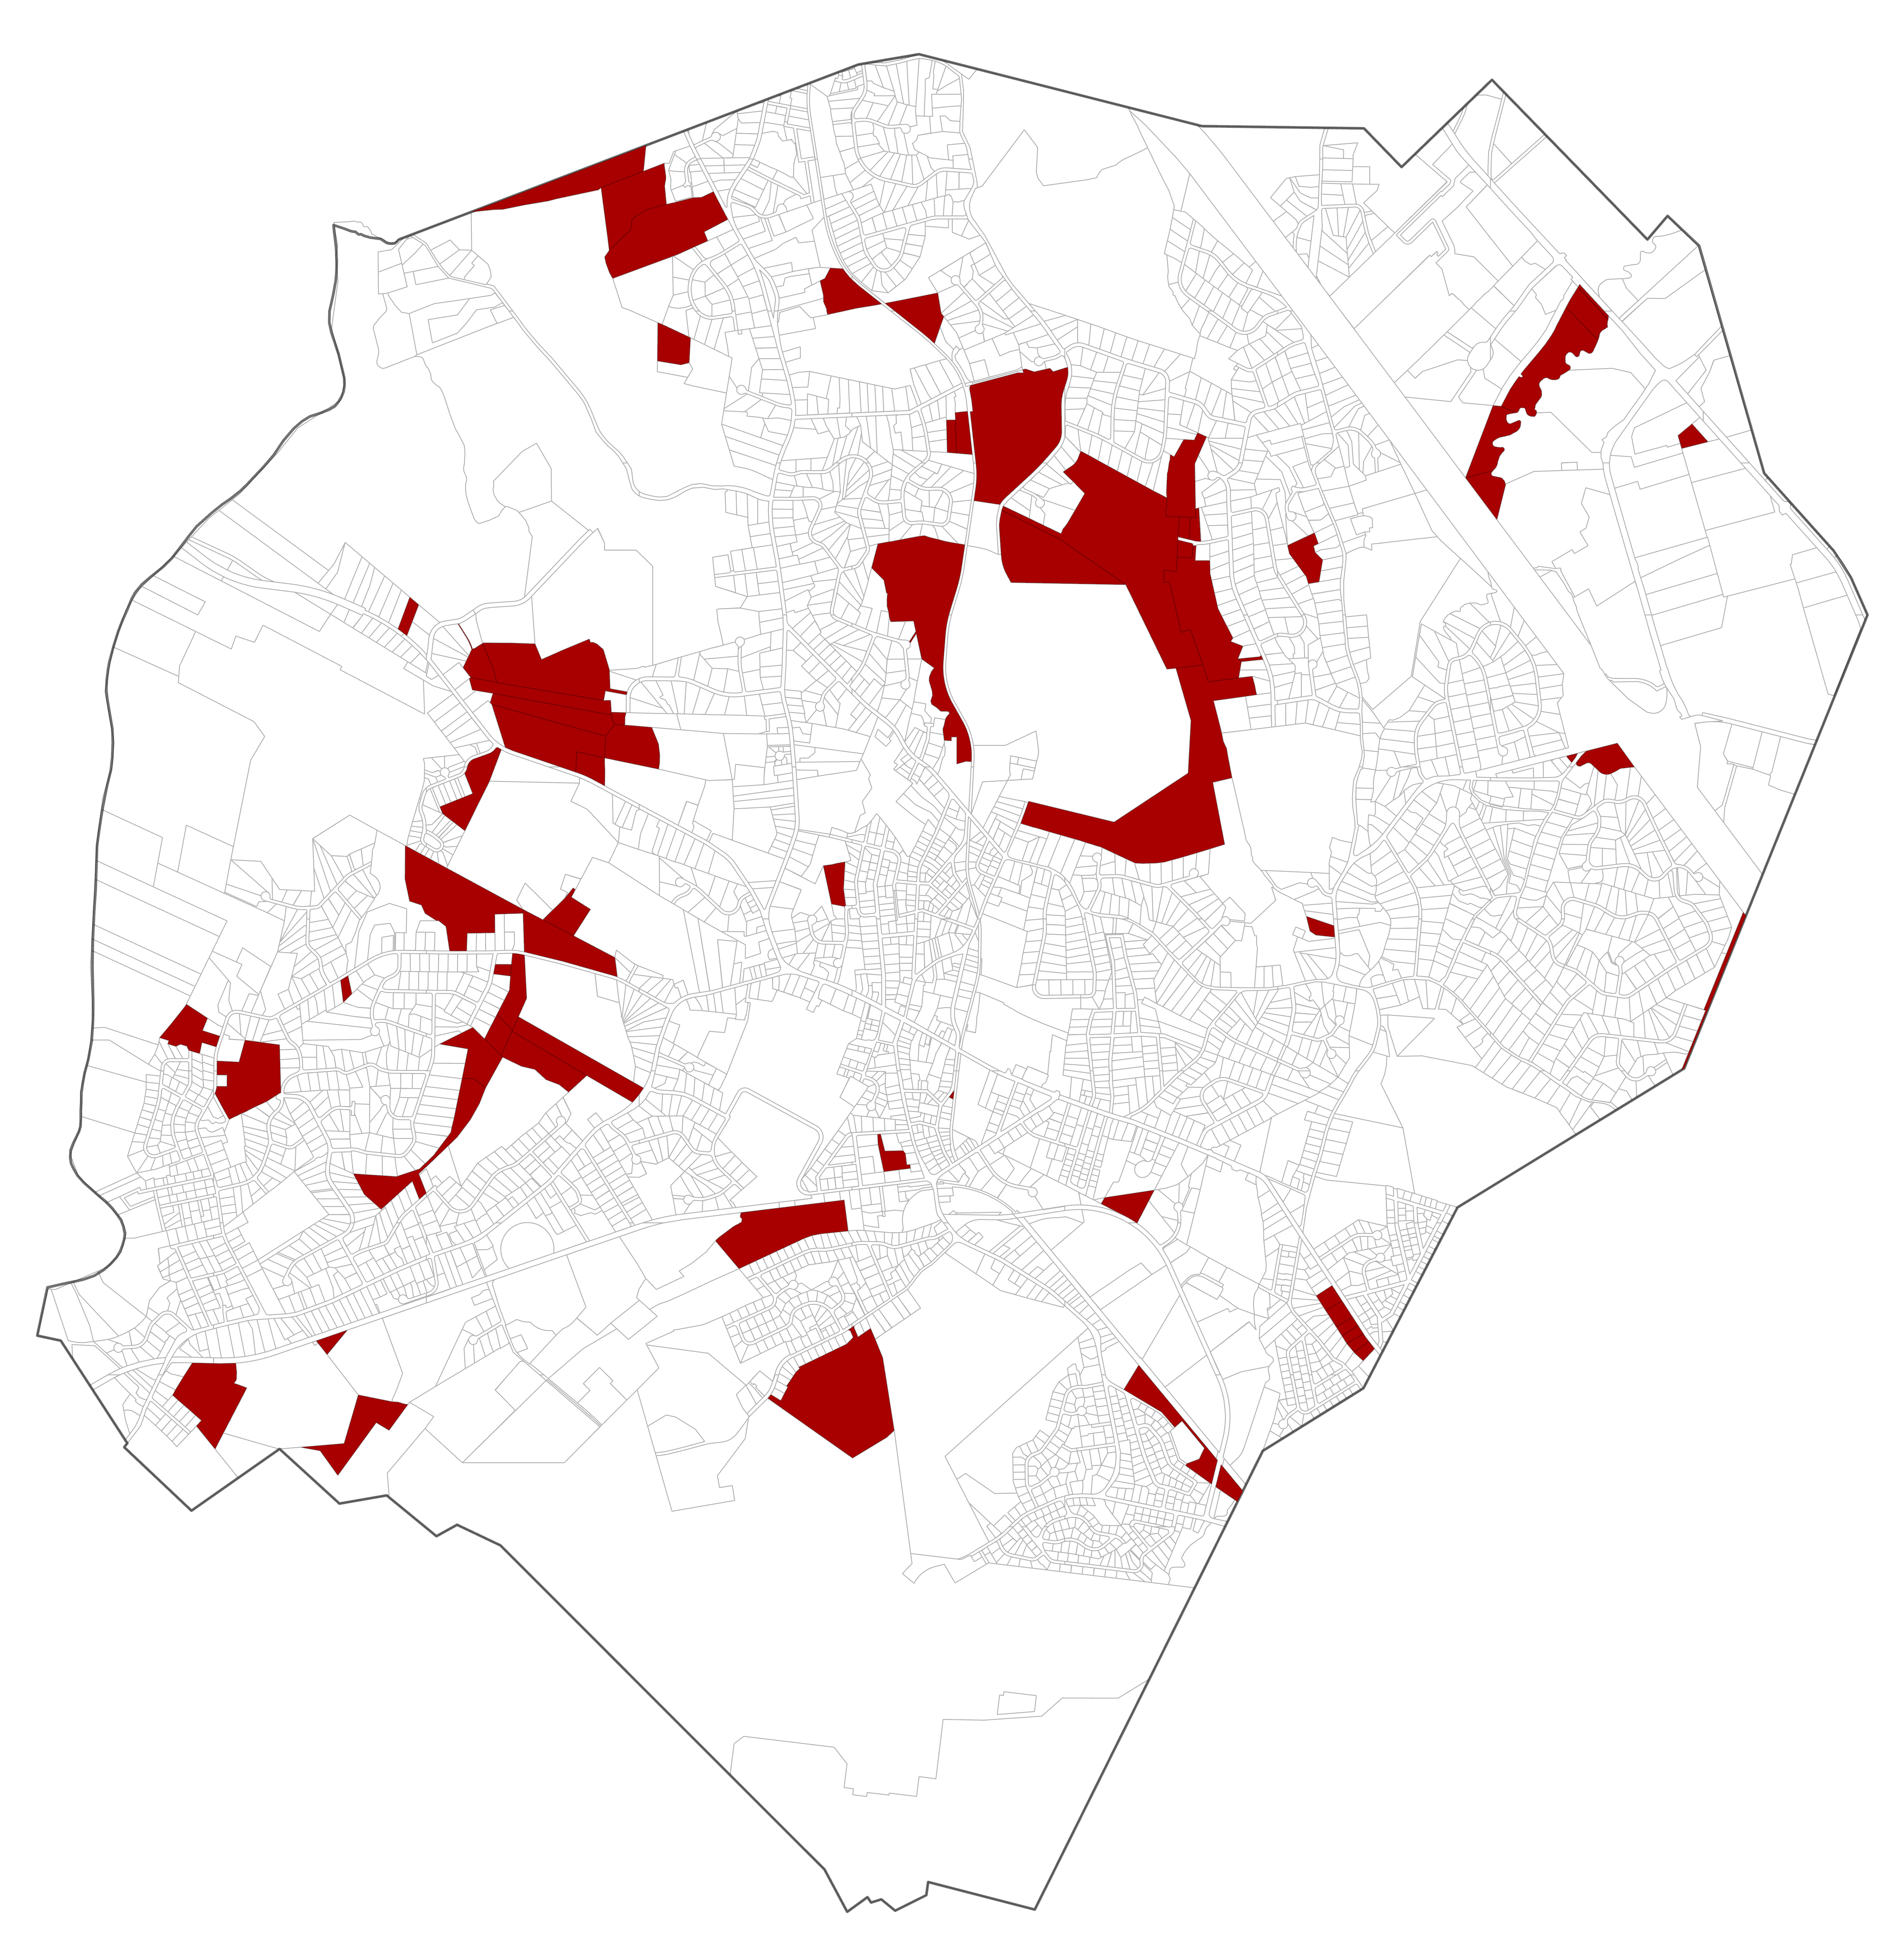
\includegraphics[width=3.64583in,height=\textheight,keepaspectratio,alt={Example map of vacant parcels identified}]{Vacant_Parcels.png}

}

\caption{\emph{Example map of vacant parcels identified}}

\end{figure}%

\textbf{Example query logic:}

\begin{Shaded}
\begin{Highlighting}[]
\NormalTok{STATE\_USE }\KeywordTok{IS} \StringTok{\textquotesingle{}\%500\%\textquotesingle{}}  
\KeywordTok{OR}\NormalTok{ STATE\_USE\_DESCRIPTION }\KeywordTok{CONTAINS} \StringTok{\textquotesingle{}\%VAC\%\textquotesingle{}}
\end{Highlighting}
\end{Shaded}

\section{Potentially Redevelopable
Land}\label{potentially-redevelopable-land}

Potentially redevelopable land consists of previously developed parcels
with characteristics suggesting they may be underutilized or suitable
for redevelopment. Consider the following approaches:

\subsection{\texorpdfstring{\textbf{Brownfields}}{Brownfields}}\label{brownfields}

\begin{quote}
Previously contaminated or industrial sites undergoing or eligible for
cleanup.
\end{quote}

The available data describing brownfield site locations is provided as
an .xlsx file maintained by the Connecticut Department of Energy \&
Environmental Protection (DEEP).

\textbf{Dataset}:
\href{https://portal.ct.gov/deep/remediation--site-clean-up/brownfields/brownfields-site-inventory}{Connecticut
Brownfields Inventory}

\begin{enumerate}
\def\labelenumi{\arabic{enumi}.}
\item
  \textbf{Spatializing the data}: Since this data is provided in a
  tabular format, it is necessary to spatialize it before processing
  with further analysis. While geocoding is feasible, it is recommended
  to use the Latitude and Longitude fields to create points
  corresponding to each brownfield site. The CRS should be NAD 83
  Connecticut State Plane (2011). The following resources provide
  details on translating the tabular latitude and longitude data into
  geospatial points:

  \begin{itemize}
  \tightlist
  \item
    ArcGIS Pro:
    \href{https://doc.esri.com/en/arcgis-pro/latest/tool-reference/data-management/xy-table-to-point.html?tabs=dialog}{XY
    Table to Point}
  \item
    QGIS:
    \href{https://qgis-tuts-wu.readthedocs.io/en/latest/land_degradation_development/interpolation/loading_table.html}{Create
    Point Layer from Table}
  \end{itemize}
\item
  Identifying brownfield parcels: Next, use the points to identify
  parcels that contain brownfield sites. This may be achieved with
  various queries, summary tools, or join tools that utilize spatial
  overlap. The following resources provide details and options for this
  process:

  \begin{itemize}
  \tightlist
  \item
    ArcGIS Pro: \hyperref[0]{Select by Location}, \hyperref[0]{Spatial
    Join}, \hyperref[0]{Summarize Within}
  \item
    QGIS: \hyperref[0]{Extract by Location} or \hyperref[0]{Select by
    Location} within Vector Selection, \hyperref[0]{Join Attributes by
    Location}
  \end{itemize}
\end{enumerate}

\begin{figure}[H]

{\centering 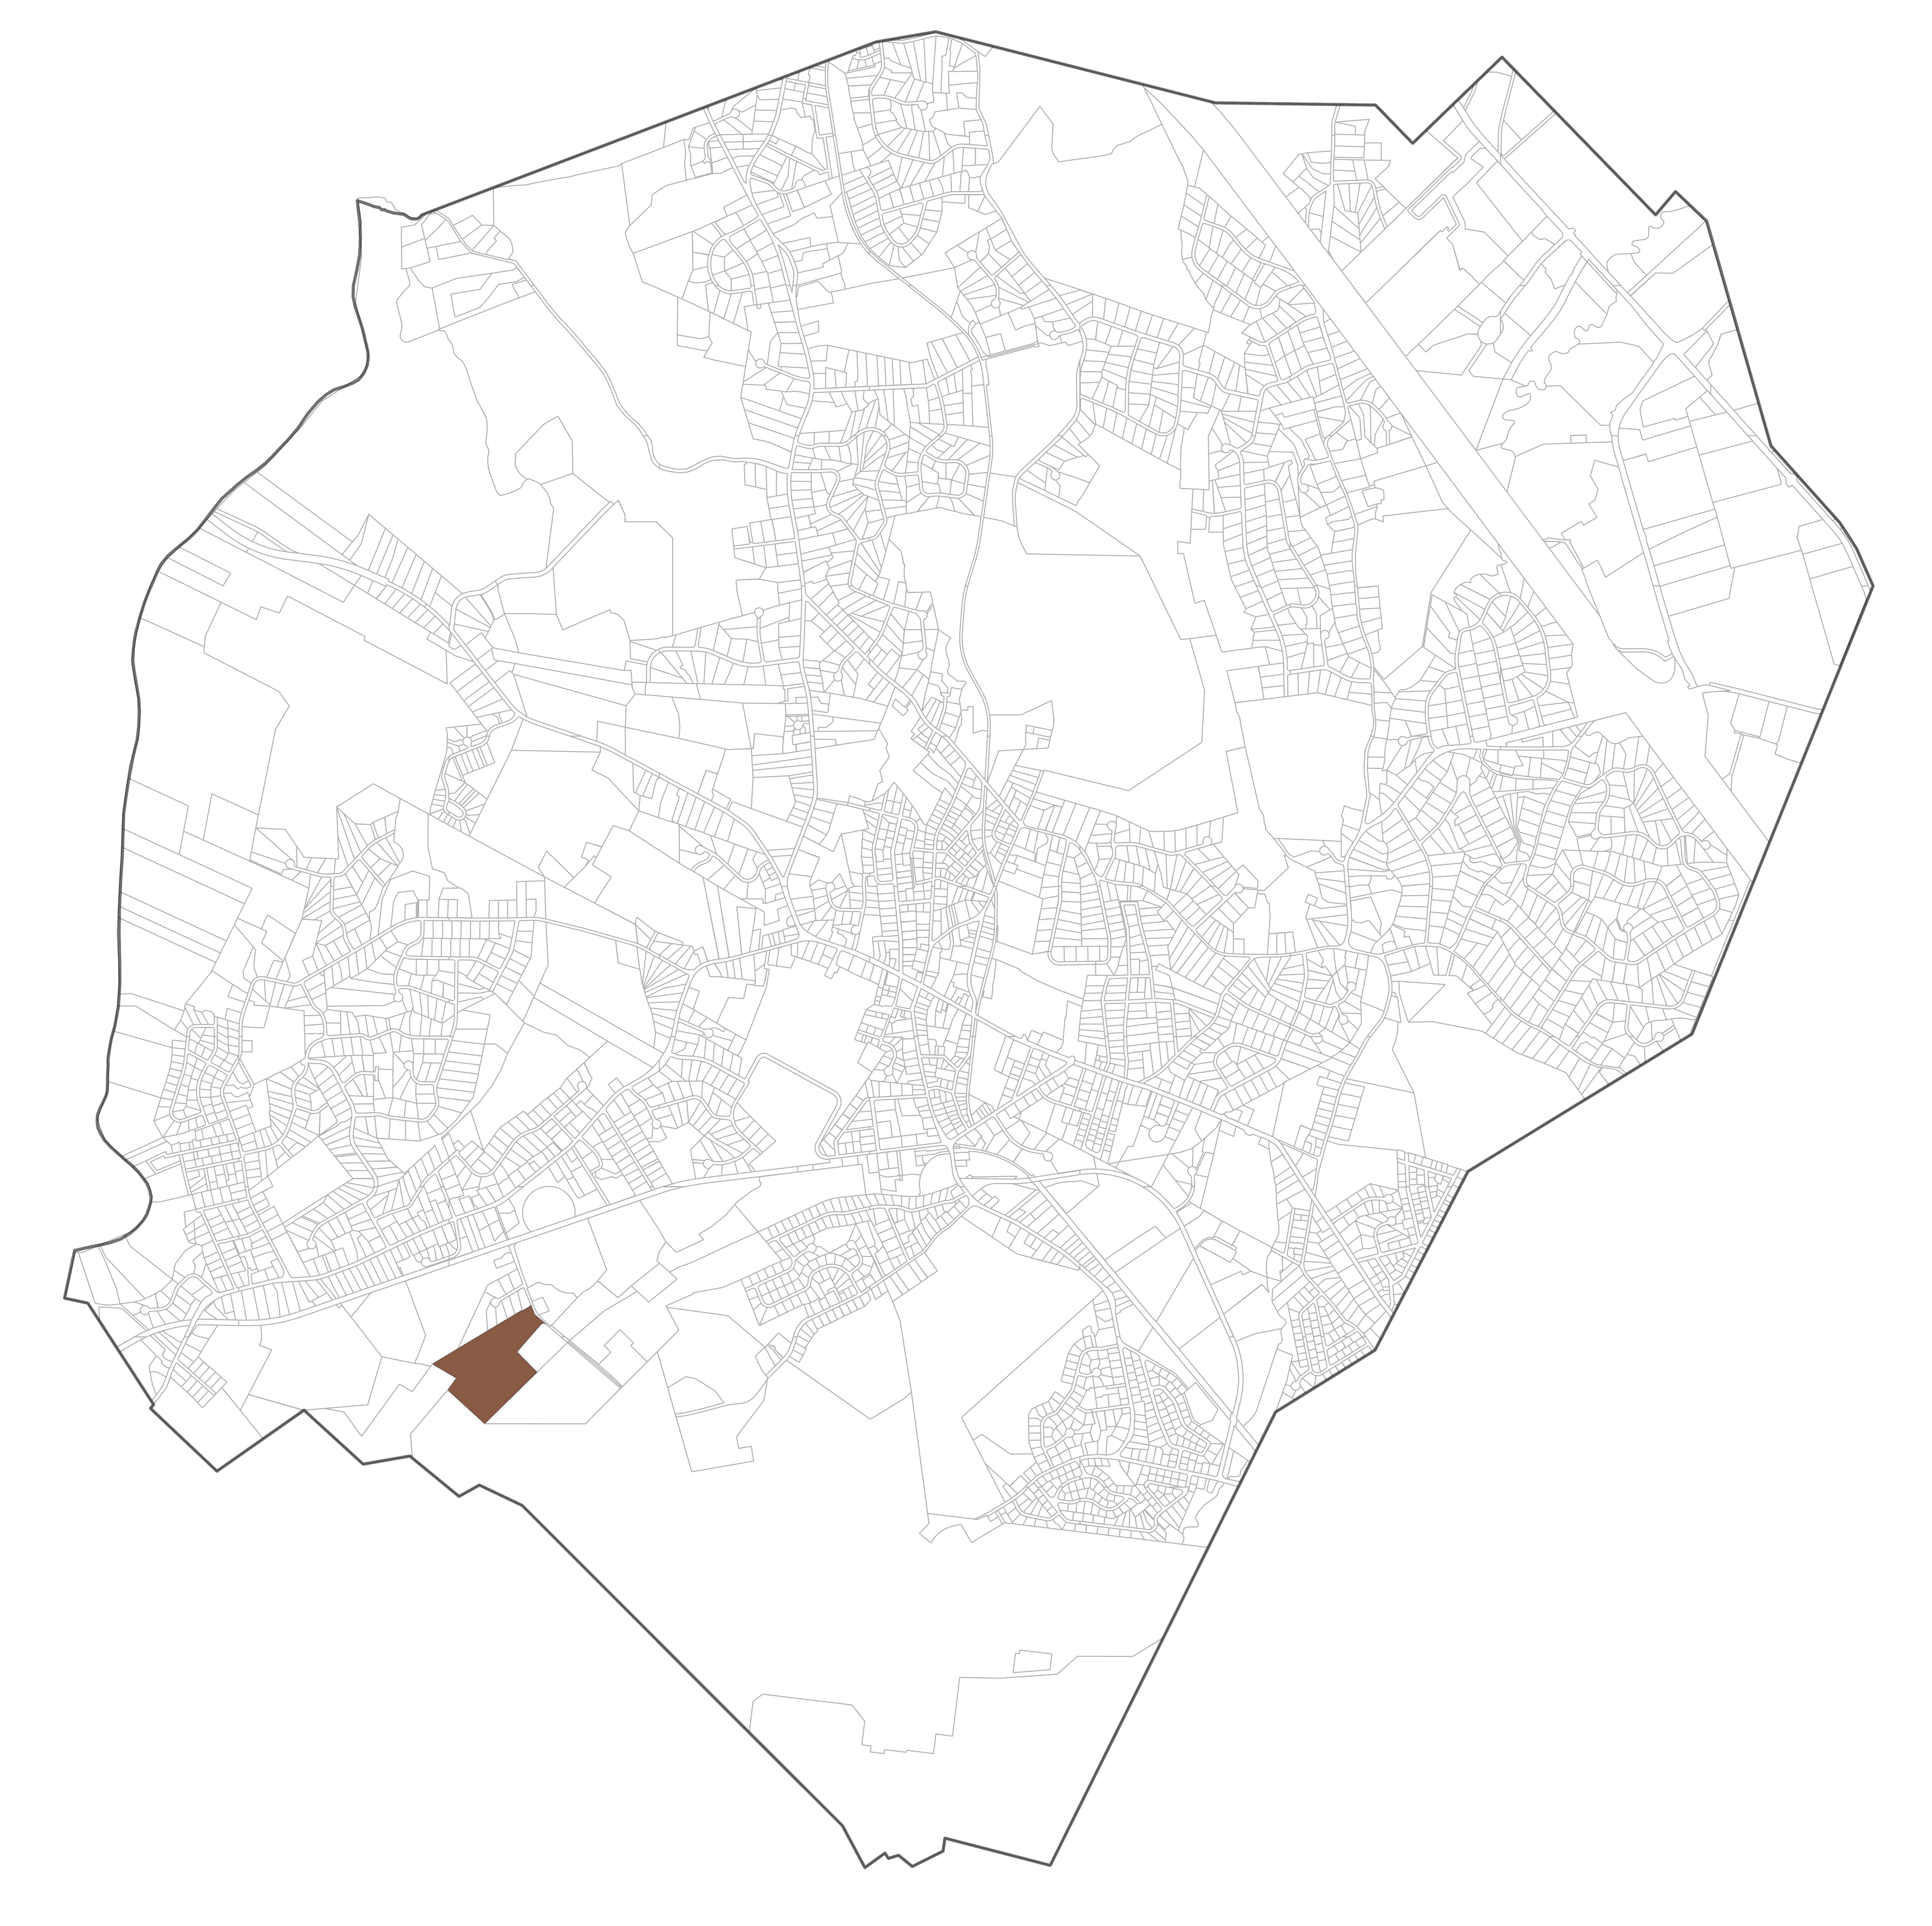
\includegraphics[width=3.64583in,height=\textheight,keepaspectratio,alt={Example map of brownfield site parcels identified}]{brownfields.png}

}

\caption{\emph{Example map of brownfield site parcels identified}}

\end{figure}%

\subsection{\texorpdfstring{\textbf{Land-to-improvement value
ratio}}{Land-to-improvement value ratio}}\label{land-to-improvement-value-ratio}

\begin{quote}
Analyze assessed land value to assessed improvements value in certain
areas or districts to identify properties that may be underperforming
(significantly higher than average land-to-improvements values)
\end{quote}

\begin{enumerate}
\def\labelenumi{\arabic{enumi}.}
\item
  \textbf{Calculating improvement values}:

  A land-to-improvement (LTI) ratio compares a parcel's appraised
  building value to the value of that parcel's land area. Parcels with
  exceptionally high LTI ratios have potential for redevelopment with
  higher-performing structures.

  Improvement value can be found by totaling the combined appraised
  value of primary buildings, outbuildings (such as sheds and detached
  garages), and extra features (such as decks and patios). In the
  \href{https://geodata.ct.gov/datasets/ctmaps::connecticut-cama-and-parcel-layer/about}{Connecticut
  CAMA and Parcel Layer}, improvement values can be calculated by
  summing the ``Appraised Building'', ``Appraised Outbuilding'', and
  ``Appraised Extra Feature'' fields. The ``Appraised Total'' field
  should not be used in this analysis, as this field represents the
  combined appraised value of improvements and land.

  \textbf{Improvement} = Appraised\_Building + Appraised\_Outbuilding +
  Appraised\_Extra\_Feature
\item
  \textbf{Calculating LTI Ratios}

  After finding the total improvement value of each parcel, a new field
  of land-to-improvement ratios can be calculated. Divide the
  ``Appraised Land'' field by the newly created improvement field.

  \textbf{LTI\_Ratio} = Appraised\_Land / Improvement
\item
  \textbf{Interpreting the LTI Ratio}
\end{enumerate}

\global\setlength{\Oldarrayrulewidth}{\arrayrulewidth}

\global\setlength{\Oldtabcolsep}{\tabcolsep}

\setlength{\tabcolsep}{2pt}

\renewcommand*{\arraystretch}{1.5}



\providecommand{\ascline}[3]{\noalign{\global\arrayrulewidth #1}\arrayrulecolor[HTML]{#2}\cline{#3}}

\begin{longtable*}[c]{|p{1.50in}|p{4.00in}}



\ascline{1.5pt}{666666}{1-2}

\multicolumn{1}{>{\centering}p{\dimexpr 1.5in+0\tabcolsep}}{\advance\leftskip by 4.0pt\relax \advance\rightskip by 4.0pt\relax \textcolor[HTML]{000000}{\fontsize{10}{10}\selectfont{{\fontspec{Arial} \textbf{LTI\ Ratio}}}}} & \multicolumn{1}{>{\centering}p{\dimexpr 4in+0\tabcolsep}}{\advance\leftskip by 4.0pt\relax \advance\rightskip by 4.0pt\relax \textcolor[HTML]{000000}{\fontsize{10}{10}\selectfont{{\fontspec{Arial} \textbf{Interpretation}}}}} \\

\ascline{1.5pt}{666666}{1-2}\endfirsthead 

\ascline{1.5pt}{666666}{1-2}

\multicolumn{1}{>{\centering}p{\dimexpr 1.5in+0\tabcolsep}}{\advance\leftskip by 4.0pt\relax \advance\rightskip by 4.0pt\relax \textcolor[HTML]{000000}{\fontsize{10}{10}\selectfont{{\fontspec{Arial} \textbf{LTI\ Ratio}}}}} & \multicolumn{1}{>{\centering}p{\dimexpr 4in+0\tabcolsep}}{\advance\leftskip by 4.0pt\relax \advance\rightskip by 4.0pt\relax \textcolor[HTML]{000000}{\fontsize{10}{10}\selectfont{{\fontspec{Arial} \textbf{Interpretation}}}}} \\

\ascline{1.5pt}{666666}{1-2}\endhead



\multicolumn{1}{>{\centering}p{\dimexpr 1.5in+0\tabcolsep}}{\advance\leftskip by 4.0pt\relax \advance\rightskip by 4.0pt\relax \textcolor[HTML]{000000}{\fontsize{10}{10}\selectfont{{\fontspec{Arial} <\ 1.0}}}} & \multicolumn{1}{>{\raggedright}p{\dimexpr 4in+0\tabcolsep}}{\advance\leftskip by 4.0pt\relax \advance\rightskip by 4.0pt\relax \textcolor[HTML]{000000}{\fontsize{10}{10}\selectfont{{\fontspec{Arial} The\ building(s)\ are\ worth\ more\ than\ the\ land}}}} \\

\ascline{0.75pt}{666666}{1-2}



\multicolumn{1}{>{\centering}p{\dimexpr 1.5in+0\tabcolsep}}{\advance\leftskip by 4.0pt\relax \advance\rightskip by 4.0pt\relax \textcolor[HTML]{000000}{\fontsize{10}{10}\selectfont{{\fontspec{Arial} =\ 1.0}}}} & \multicolumn{1}{>{\raggedright}p{\dimexpr 4in+0\tabcolsep}}{\advance\leftskip by 4.0pt\relax \advance\rightskip by 4.0pt\relax \textcolor[HTML]{000000}{\fontsize{10}{10}\selectfont{{\fontspec{Arial} Land\ and\ structures\ are\ valued\ equally}}}} \\

\ascline{0.75pt}{666666}{1-2}



\multicolumn{1}{>{\centering}p{\dimexpr 1.5in+0\tabcolsep}}{\advance\leftskip by 4.0pt\relax \advance\rightskip by 4.0pt\relax \textcolor[HTML]{000000}{\fontsize{10}{10}\selectfont{{\fontspec{Arial} >\ 1.0}}}} & \multicolumn{1}{>{\raggedright}p{\dimexpr 4in+0\tabcolsep}}{\advance\leftskip by 4.0pt\relax \advance\rightskip by 4.0pt\relax \textcolor[HTML]{000000}{\fontsize{10}{10}\selectfont{{\fontspec{Arial} The\ land\ value\ is\ equal\ to\ or\ higher\ than\ the\ improvement\ value,\ redevelopment\ may\ be\ more\ likely}}}} \\

\ascline{1.5pt}{666666}{1-2}



\end{longtable*}



\arrayrulecolor[HTML]{000000}

\global\setlength{\arrayrulewidth}{\Oldarrayrulewidth}

\global\setlength{\tabcolsep}{\Oldtabcolsep}

\renewcommand*{\arraystretch}{1}

\begin{verbatim}
Because land and improvement values vary significantly across markets, any LTI threshold used to identify underperforming parcels should be based on local market conditions and development patterns.
\end{verbatim}

\begin{figure}[H]

{\centering 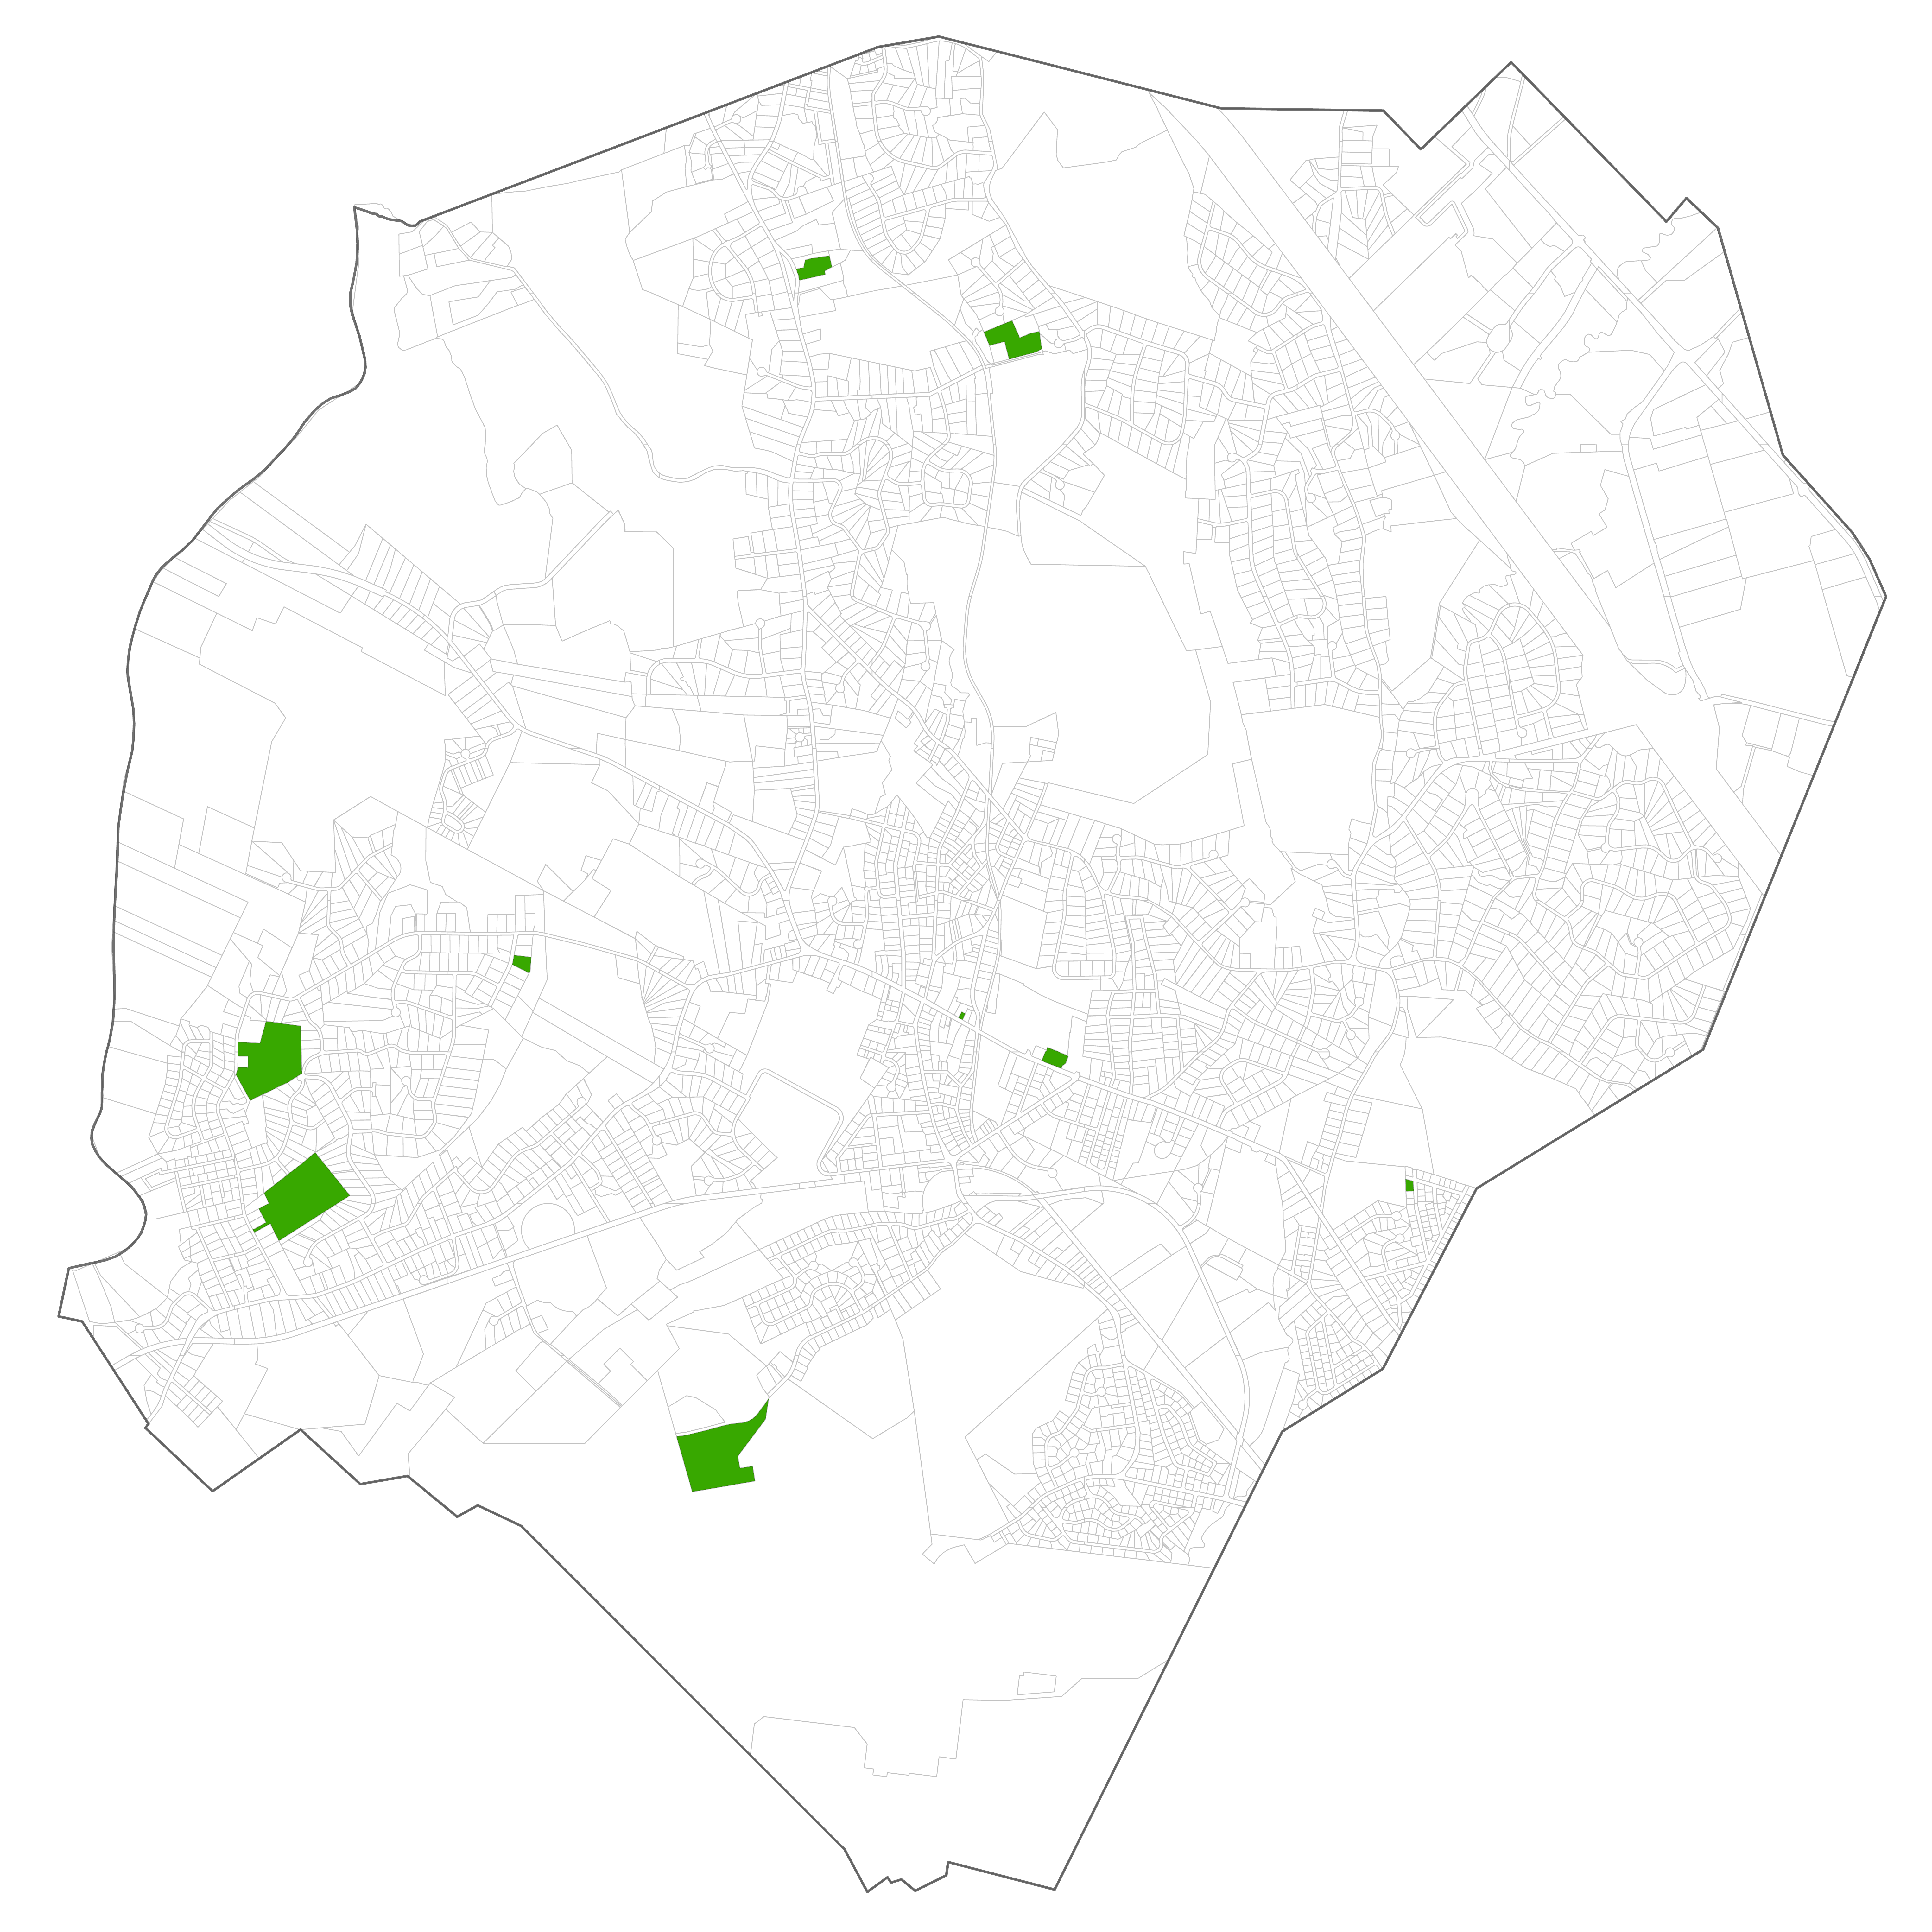
\includegraphics[width=3.64583in,height=\textheight,keepaspectratio,alt={Example map of LTI parcels identified using the applied threshold.}]{LTI_ratio.png}

}

\caption{\emph{Example map of LTI parcels identified using the applied
threshold.}}

\end{figure}%

\subsection{\texorpdfstring{\textbf{Parcel size relative to district
average}}{Parcel size relative to district average}}\label{parcel-size-relative-to-district-average}

\begin{quote}
Analyze parcel size by neighborhood or regulatory district to identify
parcels that may be underutilized (significantly larger than the
average) which may indicate an opportunity for infill development
\end{quote}

The feasibility of redevelopment efforts is also dependent on parcel
size; accordingly, potentially redevelopable land analyses may include
an inventory of parcels with the largest relative area within their
neighborhood designation.

The ``Land Acres'' field in the Statewide Parcel and CAMA dataset may
have missing or incomplete data so it is recommended to use the ``Shape
Area'' field or to derive acreage directly from the parcel geometry in
GIS.

\begin{itemize}
\item
  \textbf{Normalizing parcel area by neighborhood}

  To identify parcels that are larger than others in their neighborhood,
  an analyst should select a threshold, such as the top 10\% of parcel
  area within each neighborhood or district, to flag potential infill
  opportunities.
\end{itemize}

\begin{figure}[H]

{\centering 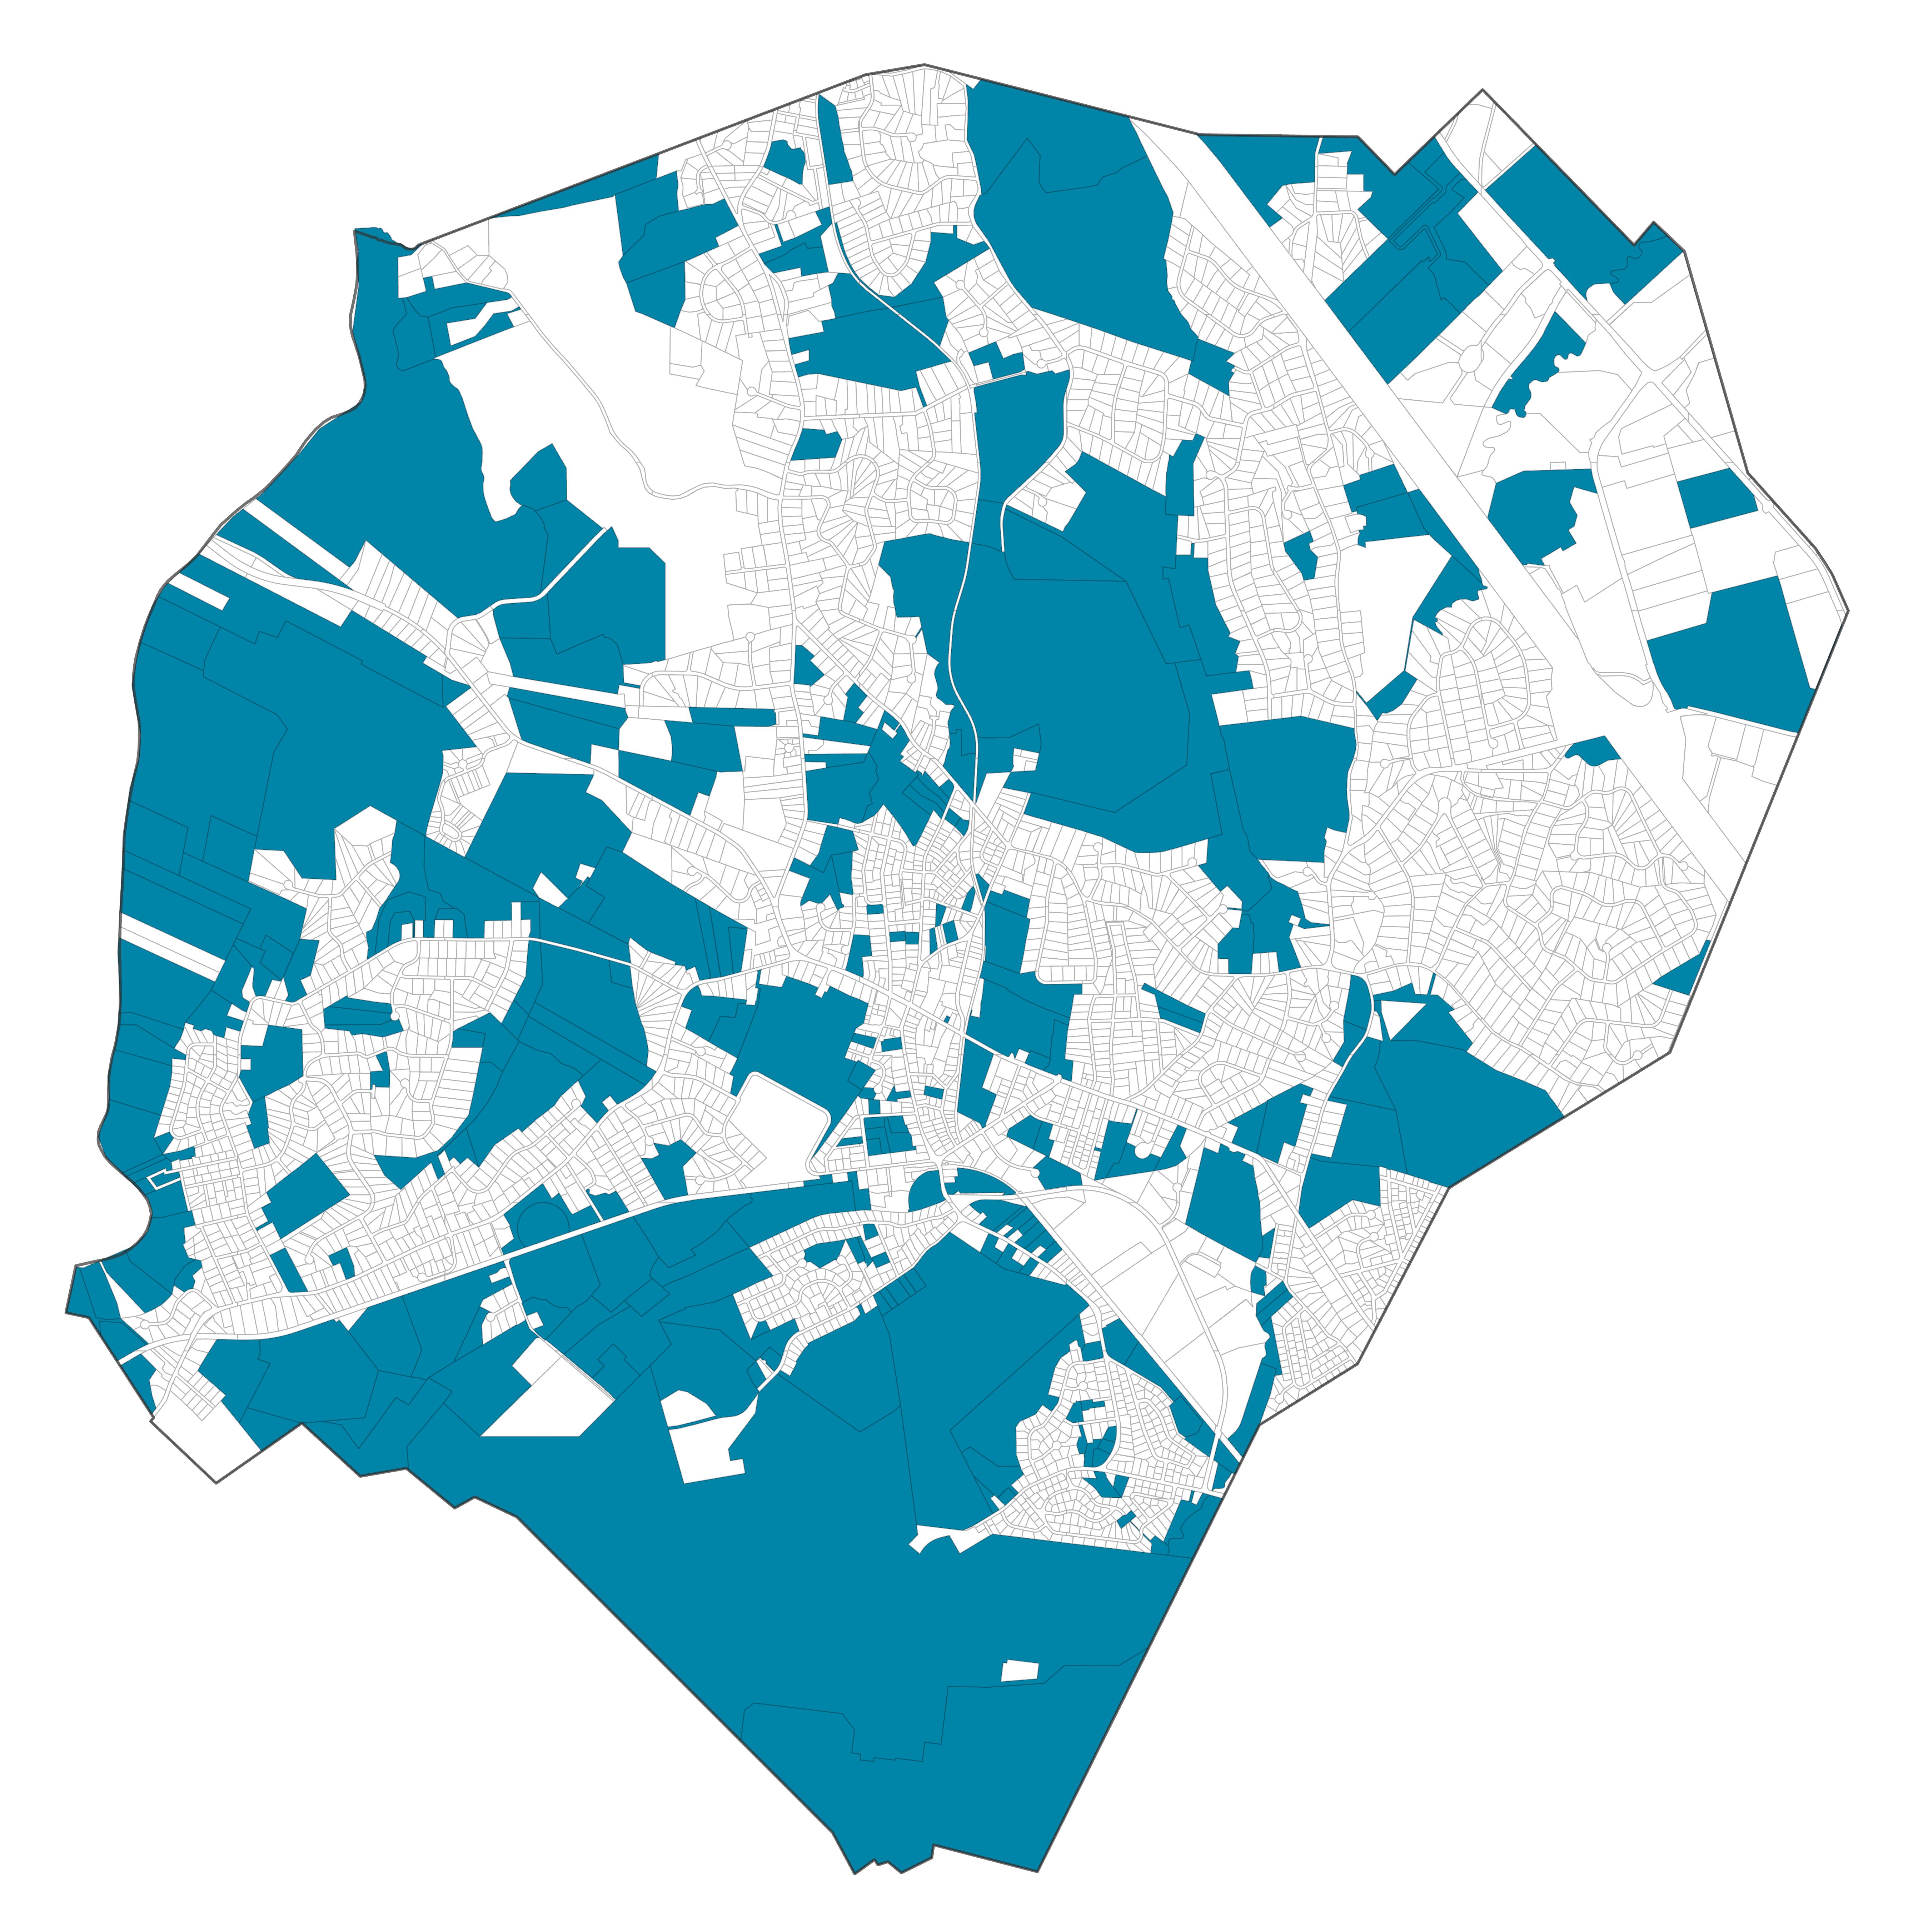
\includegraphics[width=3.64583in,height=\textheight,keepaspectratio,alt={Example map of large parcels identified.}]{Relative_Size.png}

}

\caption{\emph{Example map of large parcels identified.}}

\end{figure}%

\subsection{\texorpdfstring{\textbf{Floor Area Ratio (FAR)
analysis}}{Floor Area Ratio (FAR) analysis}}\label{floor-area-ratio-far-analysis}

\begin{quote}
Analyze Floor Area Ratios by neighborhood or district to identify
parcels that have significantly lower than average ratios which may
indicate infill or redevelopment opportunities
\end{quote}

The floor area ratio (FAR) of a parcel's primary building is the ratio
of gross building area to lot or parcel area. Higher FAR values indicate
higher building density, and lower potential for redevelopment. Whereas
land-to-improvement ratio measures the economic value of existing
buildings, the floor area ratio measures the physical space a building
occupies, weighted by number of floors.

The
\href{https://geodata.ct.gov/datasets/ctmaps::connecticut-cama-and-parcel-layer/about}{Connecticut
CAMA and Parcel Layer} field ``Gross Area of Primary Building''
represents the sum of all enclosed living and non-living building
spaces. The gross building area is measured from a building's exterior
and factors in number of floors, extending beyond the building
footprint.

In some cases, the ``Gross Area of Primary Building'' field may have
missing or incomplete data, in which case the ``Living Area'' field may
be used as a substitute. Note that this is a more restrictive metric, as
it only captures habitable, finished floor space rather than total
enclosed building area.

\begin{enumerate}
\def\labelenumi{\arabic{enumi}.}
\item
  \textbf{Calculating the FAR}

  A new field of FAR values can be calculated by dividing the ``Gross
  Area of Primary Building'' field by the parcel area field, such as the
  ``Shape Area'' field in the Connecticut CAMA and Parcel Layer.

  \textbf{FAR} = Gross Floor Area / Total Lot Area

  As previously stated, the ``Shape Area'' field or a parcel geometry
  area calculation should be used over the ``Land Acres'' field, as the
  latter may have missing or incomplete data.
\item
  \textbf{Interpreting the FAR}

  Unlike land-to-improvement ratios and relative parcel size, floor area
  ratio and potential for redevelopment have a negative relationship:
  higher FAR values indicate less possibility for redevelopment.
\end{enumerate}

\global\setlength{\Oldarrayrulewidth}{\arrayrulewidth}

\global\setlength{\Oldtabcolsep}{\tabcolsep}

\setlength{\tabcolsep}{2pt}

\renewcommand*{\arraystretch}{1.5}



\providecommand{\ascline}[3]{\noalign{\global\arrayrulewidth #1}\arrayrulecolor[HTML]{#2}\cline{#3}}

\begin{longtable*}[c]{|p{1.50in}|p{4.00in}}



\ascline{1.5pt}{666666}{1-2}

\multicolumn{1}{>{\centering}p{\dimexpr 1.5in+0\tabcolsep}}{\advance\leftskip by 4.0pt\relax \advance\rightskip by 4.0pt\relax \textcolor[HTML]{000000}{\fontsize{10}{10}\selectfont{{\fontspec{Arial} \textbf{FAR\ Ratio}}}}} & \multicolumn{1}{>{\centering}p{\dimexpr 4in+0\tabcolsep}}{\advance\leftskip by 4.0pt\relax \advance\rightskip by 4.0pt\relax \textcolor[HTML]{000000}{\fontsize{10}{10}\selectfont{{\fontspec{Arial} \textbf{Interpretation}}}}} \\

\ascline{1.5pt}{666666}{1-2}\endfirsthead 

\ascline{1.5pt}{666666}{1-2}

\multicolumn{1}{>{\centering}p{\dimexpr 1.5in+0\tabcolsep}}{\advance\leftskip by 4.0pt\relax \advance\rightskip by 4.0pt\relax \textcolor[HTML]{000000}{\fontsize{10}{10}\selectfont{{\fontspec{Arial} \textbf{FAR\ Ratio}}}}} & \multicolumn{1}{>{\centering}p{\dimexpr 4in+0\tabcolsep}}{\advance\leftskip by 4.0pt\relax \advance\rightskip by 4.0pt\relax \textcolor[HTML]{000000}{\fontsize{10}{10}\selectfont{{\fontspec{Arial} \textbf{Interpretation}}}}} \\

\ascline{1.5pt}{666666}{1-2}\endhead



\multicolumn{1}{>{\centering}p{\dimexpr 1.5in+0\tabcolsep}}{\advance\leftskip by 4.0pt\relax \advance\rightskip by 4.0pt\relax \textcolor[HTML]{000000}{\fontsize{10}{10}\selectfont{{\fontspec{Arial} <\ 1.0}}}} & \multicolumn{1}{>{\raggedright}p{\dimexpr 4in+0\tabcolsep}}{\advance\leftskip by 4.0pt\relax \advance\rightskip by 4.0pt\relax \textcolor[HTML]{000000}{\fontsize{10}{10}\selectfont{{\fontspec{Arial} The\ building's\ total\ square\ footage\ is\ smaller\ than\ the\ lot.\ This\ indicates\ low-density\ development,\ such\ as\ single-family\ homes\ or\ suburban\ subdivisions.}}}} \\

\ascline{0.75pt}{666666}{1-2}



\multicolumn{1}{>{\centering}p{\dimexpr 1.5in+0\tabcolsep}}{\advance\leftskip by 4.0pt\relax \advance\rightskip by 4.0pt\relax \textcolor[HTML]{000000}{\fontsize{10}{10}\selectfont{{\fontspec{Arial} =\ 1.0}}}} & \multicolumn{1}{>{\raggedright}p{\dimexpr 4in+0\tabcolsep}}{\advance\leftskip by 4.0pt\relax \advance\rightskip by 4.0pt\relax \textcolor[HTML]{000000}{\fontsize{10}{10}\selectfont{{\fontspec{Arial} The\ total\ building\ size\ is\ exactly\ equal\ to\ the\ lot\ size.\ This\ means\ you\ could\ build\ a\ one-story\ building\ covering\ the\ entire\ lot,\ or\ a\ two-story\ building\ covering\ half\ the\ lot.}}}} \\

\ascline{0.75pt}{666666}{1-2}



\multicolumn{1}{>{\centering}p{\dimexpr 1.5in+0\tabcolsep}}{\advance\leftskip by 4.0pt\relax \advance\rightskip by 4.0pt\relax \textcolor[HTML]{000000}{\fontsize{10}{10}\selectfont{{\fontspec{Arial} >\ 1.0}}}} & \multicolumn{1}{>{\raggedright}p{\dimexpr 4in+0\tabcolsep}}{\advance\leftskip by 4.0pt\relax \advance\rightskip by 4.0pt\relax \textcolor[HTML]{000000}{\fontsize{10}{10}\selectfont{{\fontspec{Arial} The\ building\ space\ exceeds\ the\ lot\ size,\ indicating\ multi-story,\ high-density\ development.\ For\ example,\ a\ 10-story\ building\ occupying\ 10\%\ of\ a\ lot\ yields\ a\ high\ FAR.}}}} \\

\ascline{1.5pt}{666666}{1-2}



\end{longtable*}



\arrayrulecolor[HTML]{000000}

\global\setlength{\arrayrulewidth}{\Oldarrayrulewidth}

\global\setlength{\tabcolsep}{\Oldtabcolsep}

\renewcommand*{\arraystretch}{1}

\begin{verbatim}
To identify underperforming parcels using FAR, select a threshold at the lower end of the distribution, such as parcels in the bottom 10% of FAR values within a neighborhood or district, as these represent properties where the built floor area is small relative to the land area, suggesting potential for more intensive development.
\end{verbatim}

\begin{verbatim}
::: {style="text-align:center;"}
![*Example map identifying parcels based on low FAR values.*](FAR.png){fig-alt="Example map identifying parcels based on low FAR values." width="350"}
:::
\end{verbatim}

\subsection{\texorpdfstring{\textbf{Construction and renovation year
clustering}}{Construction and renovation year clustering}}\label{construction-and-renovation-year-clustering}

\begin{quote}
Analyze construction and renovation years to identify clusters of
existing units in need of rehabilitation.
\end{quote}

Construction and renovation year clustering offers insight into building
aging patterns within municipalities, with the goal of identifying
parcel clusters that may need rehabilitation.

The
\href{https://geodata.ct.gov/datasets/ctmaps::connecticut-cama-and-parcel-layer/about}{Connecticut
CAMA and Parcel Layer} has multiple fields relevant to this analysis.

\begin{itemize}
\tightlist
\item
  ``AYB'' (Actual Year Built) field: The original construction date for
  each parcel's primary building
\item
  ``EYB'' (Effective Year Built) field: The building's effective age,
  factoring in remodeling and renovations.
\item
  ``Depreciation'' field: Percent values indicating the amount of
  depreciation a building has experienced.
\end{itemize}

It is important to note that there are no statewide criteria for
evaluating Effective Year Built. The calculation of effective building
age may vary depending on the individual judgement of assessors and is a
form of subjective data. Accordingly, if the AYB and EYB fields lack
sufficient data or if municipalities have their own criteria for
evaluating EYB, they may elect to use their own assessor data and
property records.

\begin{enumerate}
\def\labelenumi{\arabic{enumi}.}
\item
  \textbf{Construction and renovation year clustering analysis}

  This analysis uses a multivariate clustering tool in GIS to group
  parcels based on three fields simultaneously: original construction
  date (AYB), effective building age (EYB), and physical deterioration
  (Depreciation). Rather than applying a single threshold to one
  variable, multivariate clustering evaluates all three fields at once,
  automatically grouping parcels that share similar combinations of age,
  renovation history, and condition. The result is multiple groups of
  parcels, one of which will represent the oldest, least-renovated, and
  most deteriorated buildings in the study area, which are the parcels
  most likely to be candidates for rehabilitation or redevelopment

  \textbf{Why multivariate clustering?}

  A simple threshold approach (for example, filtering only by
  construction year) would miss properties that are old but have been
  well-maintained, or flag properties that are deteriorated but have
  been recently renovated. A multivariate analysis using the ``AYB'',
  ``EYB'', and ``Depreciation'' fields together can be used to flag
  groups of parcels with high redevelopment potential.

  It is also important to use a clustering method that does not rely on
  spatial relationships between parcels, meaning one that groups parcels
  based purely on shared traits rather than proximity or adjacency.
  Spatial clustering methods, such as K-nearest neighbor (KNN) or Queen
  contiguity, which would traditionally be used for parcel data using
  polygon geometry, identify parcels based on how close they are to each
  other or whether they share edges or corners. Because the parcel layer
  may be segmented by missing data, these methods will fail or produce
  inaccurate clusters by attempting to connect parcels across large
  gaps. Instead, a non-spatial multivariate clustering tool ensures that
  all parcels with available data are assigned to a cluster with shared
  features, regardless of where they are located. For more insight into
  these methods and their limitations:

  \begin{itemize}
  \tightlist
  \item
    Brief introduction to concepts, with R examples:
    \href{https://cran.r-project.org/web/packages/geostan/vignettes/spatial-weights-matrix.html}{Spatial
    Weights Matrix}
  \item
    Description of spatial statistics:
    \href{https://doc.esri.com/en/arcgis-pro/latest/tool-reference/spatial-statistics/modeling-spatial-relationships.html}{Modeling
    Spatial Relationships}
  \item
    Overview of ESRI clustering tools and their applications:
    \href{https://doc.esri.com/en/arcgis-pro/latest/tool-reference/spatial-statistics/an-overview-of-the-mapping-clusters-toolset.html}{Mapping
    Clusters}
  \end{itemize}

  Instead, it is recommended to use a multivariate clustering tool that
  relies only on the presence of shared traits. These tools identify
  optimized seed locations, or initial parcels, by maximizing their
  initial distance from each other, then repeatedly adjust these seeds
  to minimize variability within clusters and increase variability
  between clusters. In this way, all parcels with available data are
  assigned to a cluster with shared features. Simplified, the process
  is:

  \emph{assign seeds → recompute and adjust seed location → repeat until
  stable}

  The following tools and settings are recommended for conducting this
  analysis in GIS software:

  \begin{itemize}
  \tightlist
  \item
    ArcGIS Pro:
    \href{https://doc.esri.com/en/arcgis-pro/latest/tool-reference/spatial-statistics/multivariate-clustering.html?tabs=dialog}{Multivariate
    Clustering}
  \item
    QGIS:
    \href{https://knowyourspace.dk/2021/04/09/using-the-attribute-based-clustering-plugin-qgis/}{Attribute
    Based Clustering Plugin}
  \end{itemize}

  Recommended settings:

  \begin{itemize}
  \tightlist
  \item
    K-means algorithm
  \item
    4 seeds (producing 4 clusters)
  \item
    Optimized seeds
  \end{itemize}

  For the ArcGIS Pro tool, there is an option to choose between the
  K-means or K-medoids algorithm. K-medoids is robust to outliers, while
  K-means is faster and operates more efficiently with large datasets;
  accordingly, K-means is the recommended algorithm for this analysis
  and is also the default option for the QGIS Attribute Based Clustering
  Plugin.
\item
  \textbf{Data preparation}

  Within the Statewide Parcel and CAMA data, the AYB and EYB fields may
  include null placeholder values of 0, 15, or other extremely low
  numbers. Placeholders may also take the form of years from the 1500s,
  1600s, or 1700s. Accordingly, municipalities should evaluate the
  distribution of AYB values in their CAMA data, identify any outliers
  or apparent null placeholders, verify these against their oldest
  historical buildings, and filter this data out prior to running the
  clustering analysis.

  Example filter queries include:

  \begin{itemize}
  \tightlist
  \item
    ``EYB'' is not equal to 0
  \item
    ``AYB'' is greater than or equal to 1639 (the construction year of
    the Henry Whitfield House, the oldest standing building in
    Connecticut)
  \item
    ``AYB'' \textgreater= 1788 (the year of Connecticut's founding as a
    state)
  \item
    ``AYB'' \textgreater= 1899 (a common placeholder year, as it is the
    zero date in systems like SQL, Power BI, and SharePoint)
  \end{itemize}
\item
  Interpreting results

  Below is a sample series of boxplots automatically produced by running
  the Multivariate Clustering tool in ArcGIS Pro. These boxplots
  illustrate the distribution of data for the three fields of interest
  and reveal which clusters contain the combination of traits most
  relevant to this analysis. The target cluster will exhibit the lowest
  AYB, lowest EYB, and highest depreciation percentage.

  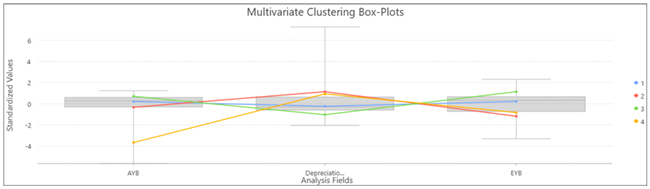
\includegraphics[width=8.33333in,height=\textheight,keepaspectratio]{mc_boxplot.png}

  For example, the yellow cluster (cluster 4) contains parcels with
  extremely low AYB, high depreciation percentage, and low EYB, while
  the red cluster (cluster 2) contains parcels with low AYB, the highest
  depreciation, and the lowest EYB. Accordingly, clusters 2 and 4 are
  groups of interest for potential rehabilitation; in this case, cluster
  2 would be isolated and included in a Potentially Redevelopable Land
  inventory, as it has the highest depreciation and lowest EYB.

  Note that AYB will naturally contain lower values than EYB, as it
  reflects original construction rather than effective age. The oldest
  buildings may have already undergone extensive renovation and
  therefore may not exhibit similarly extreme Depreciation or EYB
  values. Accordingly, Depreciation and EYB should be weighted more
  heavily when deciding which cluster to isolate, as these variables
  better reflect the current physical condition of properties.

  The figure on the left (a) shows the results of the Multivariate
  Clustering tool in ArcGIS Pro, where cluster colors on the map
  correspond to those shown in the boxplots. The figure on the right (b)
  shows the resulting map after isolating cluster 2, which represents
  the end product of a construction and renovation year clustering
  analysis.
\end{enumerate}

\begin{figure}

\begin{minipage}[t]{0.50\linewidth}

\begin{figure}[H]

{\centering \includegraphics[width=3.125in,height=\textheight,keepaspectratio,alt={multivariate clustering box plot example}]{MultiVar.png}

}

\subcaption{a) Multivariate Clustering results}

\end{figure}%

\end{minipage}%
%
\begin{minipage}[t]{0.50\linewidth}

\begin{figure}[H]

{\centering 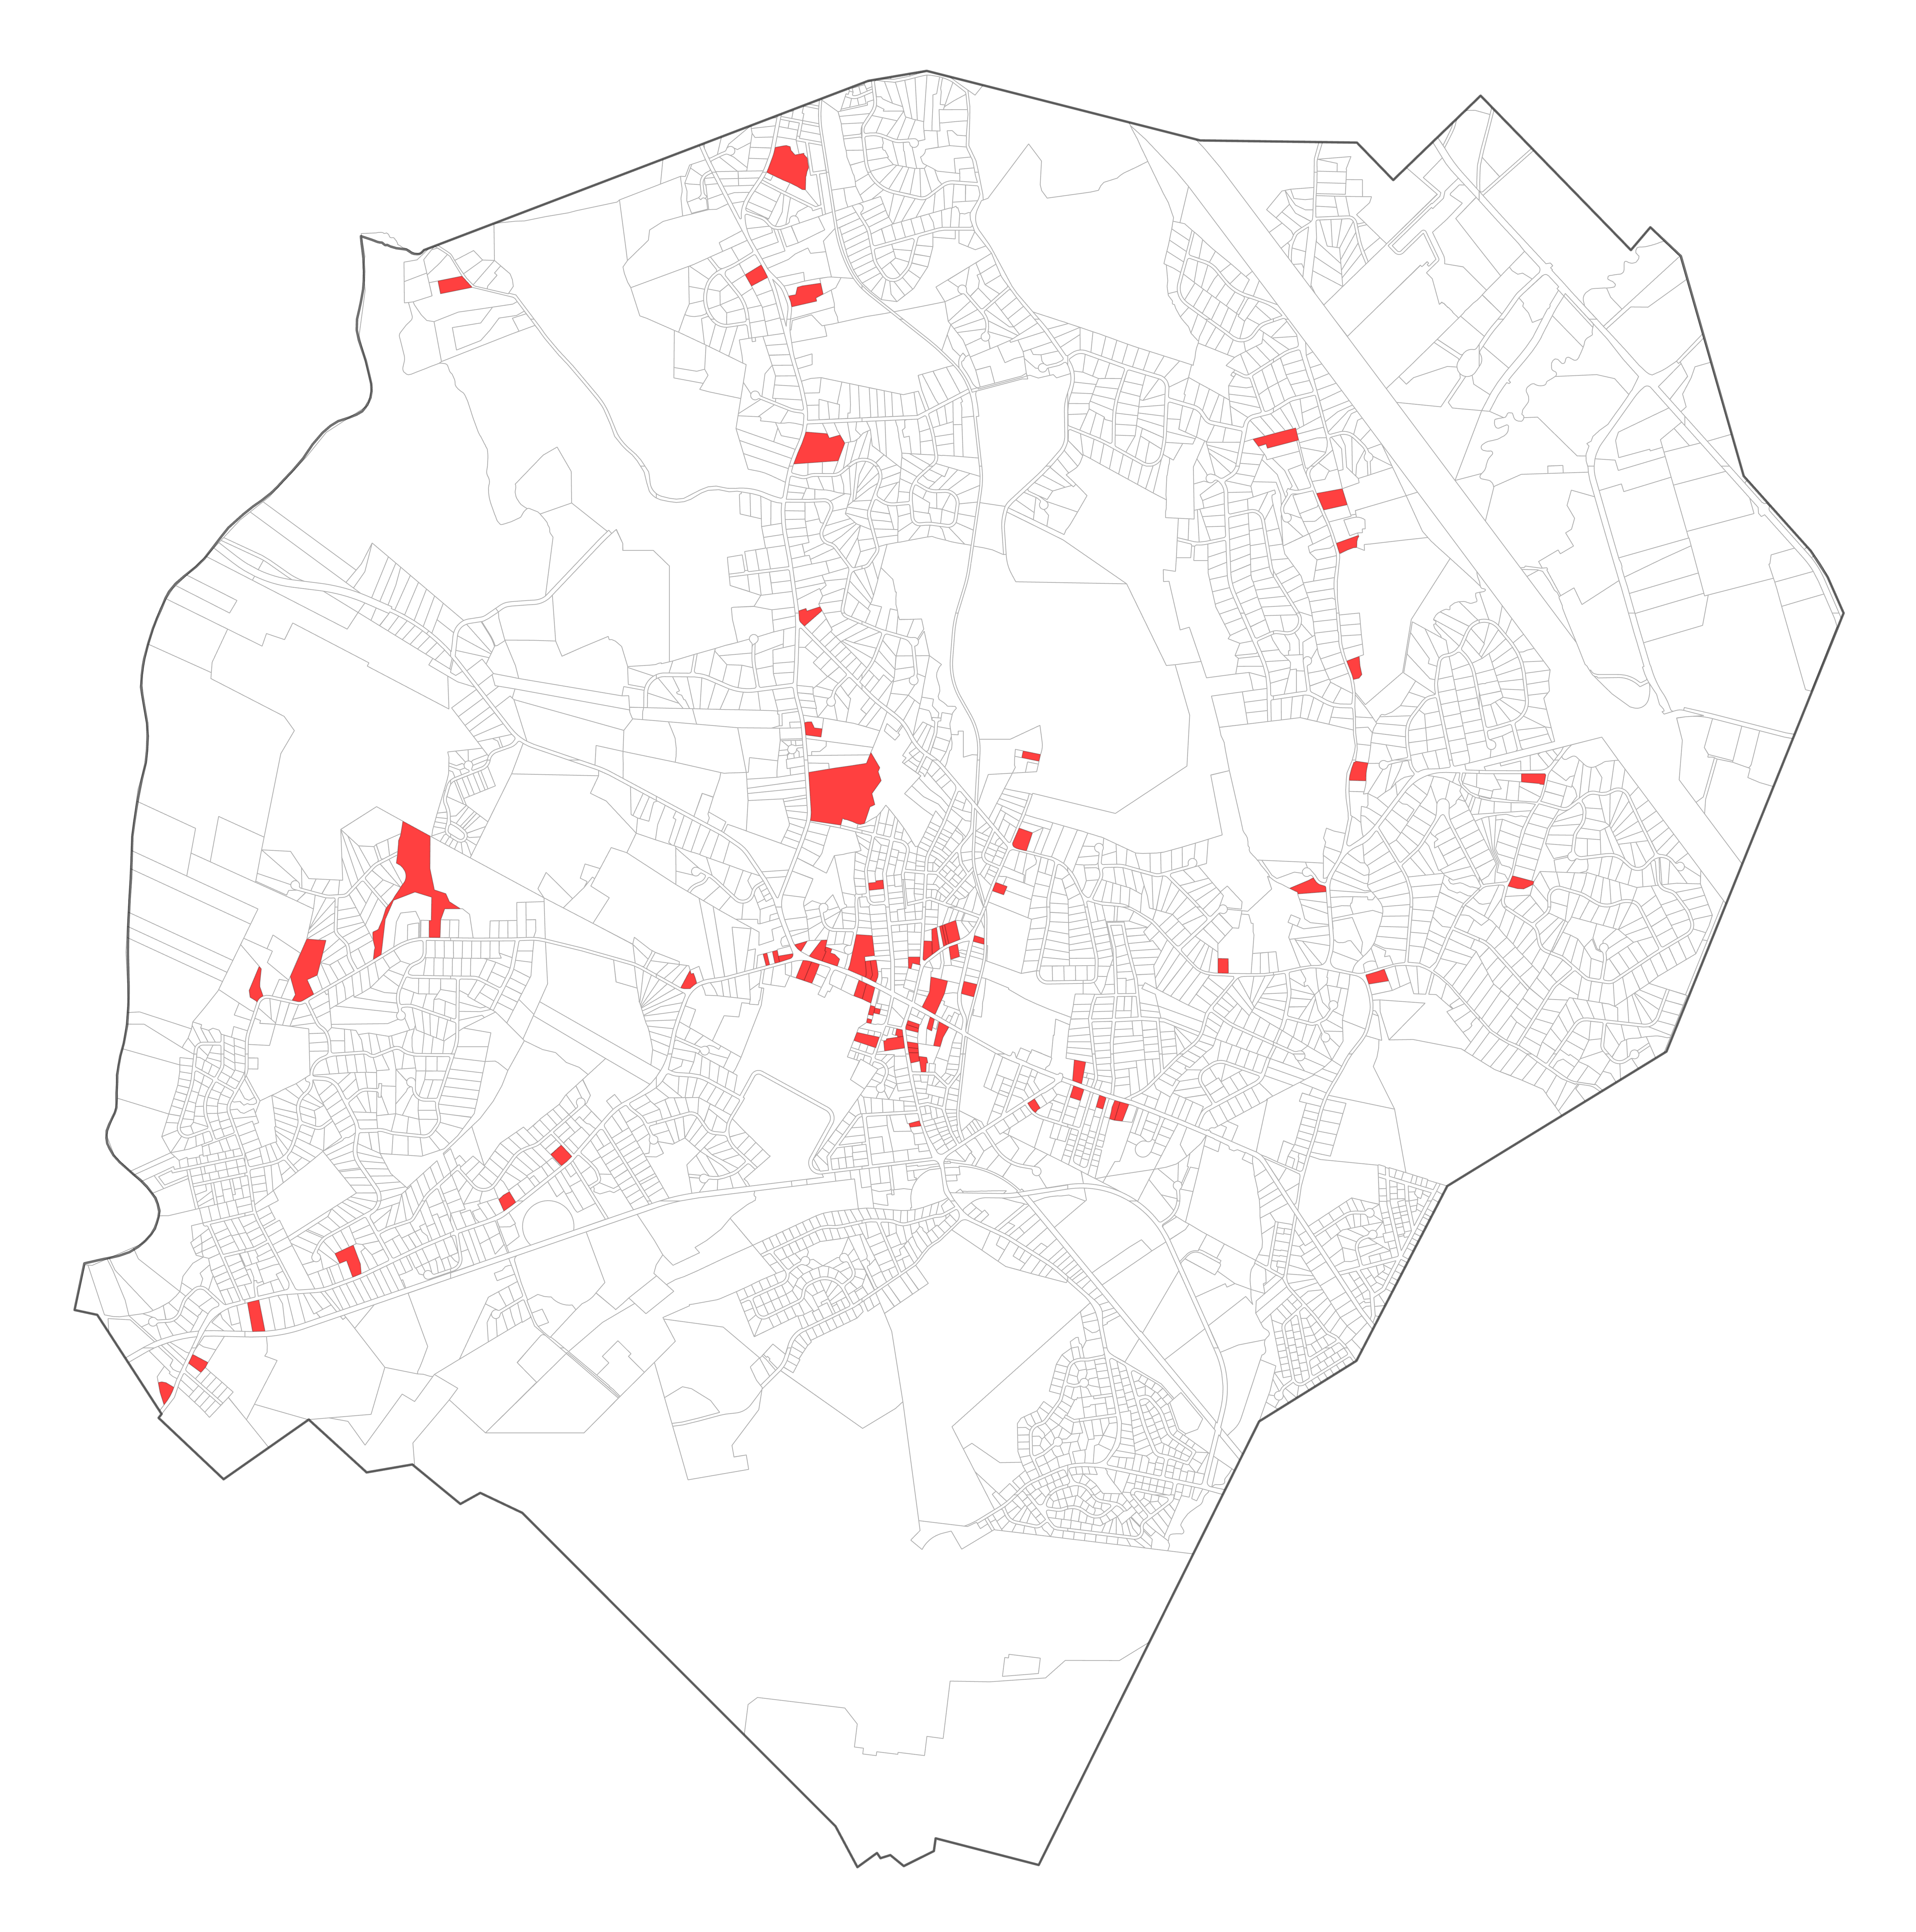
\includegraphics[width=3.125in,height=\textheight,keepaspectratio,alt={multivariate clustering box plot example}]{MultiVar2.png}

}

\subcaption{b) Cluster 2 isolated}

\end{figure}%

\end{minipage}%

\end{figure}%

\bookmarksetup{startatroot}

\chapter{Creating the Maps}\label{creating-the-maps}

The developable land inventory identifies land that meets the statutory
definition of developable land under PA 25-1. This inventory serves as a
foundational input to subsequent phases of the Housing Growth Plan
process, including the suitability analysis {[}link{]} and the parcel
and zone identification. These later steps incorporate additional
planning considerations, local context, and policy objectives to
evaluate where housing growth and affordable housing opportunities may
be most appropriate.

To support Housing Growth Plan reporting and review, the developable
land inventory should be presented in the report as municipality-wide
maps. The maps should clearly display the location and distribution of
developable land using clear, accessible, and consistent symbology.

The maps should incorporate the following data:

\begin{itemize}
\tightlist
\item
  Land identified as excluded from developable land
  (\hyperref[sec-statutory-exclusions]{Section 3})
\item
  Identified vacant parcels
  (\hyperref[identifying-vacant-and-potential-land-for-redevelopment]{Section
  4})
\item
  Identified parcels with redevelopment potential
  (\hyperref[identifying-vacant-and-potential-land-for-redevelopment]{Section
  4})
\end{itemize}

The final maps included in the Housing Growth Plan will be:

\begin{enumerate}
\def\labelenumi{\arabic{enumi}.}
\tightlist
\item
  \textbf{Statutory Exclusions Map}: A municipality-wide map displaying
  each statutory exclusion category as a separate layer and symbolized
  distinctly to illustrate the distribution of land excluded from the
  developable land inventory.
\item
  \textbf{Developable vs.~Non-Developable Land Map}: A municipality-wide
  map depicting all statutory exclusion categories combined into a
  single consolidated layer symbolized as non-developable land. All
  remaining land not subject to statutory exclusions is displayed as
  developable land, providing a simplified binary representation of land
  suitability across the municipality.
\item
  \textbf{Developable Land Summary Map}: A municipality-wide map
  displaying all statutory exclusion categories combined into a single
  exclusion layer, alongside a developable land layer representing all
  land remaining after the exclusion analysis. Identified vacant parcels
  and parcels with redevelopment potential should be displayed as
  separate overlays.
\end{enumerate}

\section{Map Layers and Symbology}\label{map-layers-and-symbology}

All maps include the municipal boundary layer to delineate the
geographic extent of the study area.

\textbf{Dataset}:
\href{https://geodata.ct.gov/datasets/ctmaps::ct-municipalities-with-fips/about}{CT
Municipalities (CT Geodata Portal)}

Municipal parcel boundaries are included where appropriate to provide
spatial context for interpretation of mapped datasets.

\textbf{Dataset}:
\href{https://geodata.ct.gov/datasets/ctmaps::connecticut-cama-and-parcel-layer/about}{Connecticut
CAMA and Parcel Layer (CT Geodata Portal)}

\begin{enumerate}
\def\labelenumi{\arabic{enumi}.}
\tightlist
\item
  \textbf{Statutory Exclusions Map}
\end{enumerate}

\global\setlength{\Oldarrayrulewidth}{\arrayrulewidth}

\global\setlength{\Oldtabcolsep}{\tabcolsep}

\setlength{\tabcolsep}{2pt}

\renewcommand*{\arraystretch}{1.5}



\providecommand{\ascline}[3]{\noalign{\global\arrayrulewidth #1}\arrayrulecolor[HTML]{#2}\cline{#3}}

\begin{longtable*}[c]{|p{2.80in}|p{2.20in}|p{1.50in}}



\ascline{1.5pt}{666666}{1-3}

\multicolumn{1}{>{\raggedright}p{\dimexpr 2.8in+0\tabcolsep}}{\advance\leftskip by 4.0pt\relax \advance\rightskip by 4.0pt\relax \textcolor[HTML]{000000}{\fontsize{10}{10}\selectfont{{\fontspec{Arial} \textbf{Map\ Layer\ (top\ to\ bottom)}}}}} & \multicolumn{1}{>{\raggedright}p{\dimexpr 2.2in+0\tabcolsep}}{\advance\leftskip by 4.0pt\relax \advance\rightskip by 4.0pt\relax \textcolor[HTML]{000000}{\fontsize{10}{10}\selectfont{{\fontspec{Arial} \textbf{Description}}}}} & \multicolumn{1}{>{\raggedright}p{\dimexpr 1.5in+0\tabcolsep}}{\advance\leftskip by 4.0pt\relax \advance\rightskip by 4.0pt\relax \textcolor[HTML]{000000}{\fontsize{10}{10}\selectfont{{\fontspec{Arial} \textbf{Recommended\ Symbology}}}}} \\

\ascline{1.5pt}{666666}{1-3}\endfirsthead 

\ascline{1.5pt}{666666}{1-3}

\multicolumn{1}{>{\raggedright}p{\dimexpr 2.8in+0\tabcolsep}}{\advance\leftskip by 4.0pt\relax \advance\rightskip by 4.0pt\relax \textcolor[HTML]{000000}{\fontsize{10}{10}\selectfont{{\fontspec{Arial} \textbf{Map\ Layer\ (top\ to\ bottom)}}}}} & \multicolumn{1}{>{\raggedright}p{\dimexpr 2.2in+0\tabcolsep}}{\advance\leftskip by 4.0pt\relax \advance\rightskip by 4.0pt\relax \textcolor[HTML]{000000}{\fontsize{10}{10}\selectfont{{\fontspec{Arial} \textbf{Description}}}}} & \multicolumn{1}{>{\raggedright}p{\dimexpr 1.5in+0\tabcolsep}}{\advance\leftskip by 4.0pt\relax \advance\rightskip by 4.0pt\relax \textcolor[HTML]{000000}{\fontsize{10}{10}\selectfont{{\fontspec{Arial} \textbf{Recommended\ Symbology}}}}} \\

\ascline{1.5pt}{666666}{1-3}\endhead



\multicolumn{1}{>{\raggedright}p{\dimexpr 2.8in+0\tabcolsep}}{\advance\leftskip by 4.0pt\relax \advance\rightskip by 4.0pt\relax \textcolor[HTML]{000000}{\fontsize{10}{10}\selectfont{{\fontspec{Arial} Municipality\ boundary}}}} & \multicolumn{1}{>{\raggedright}p{\dimexpr 2.2in+0\tabcolsep}}{\advance\leftskip by 4.0pt\relax \advance\rightskip by 4.0pt\relax \textcolor[HTML]{000000}{\fontsize{10}{10}\selectfont{{\fontspec{Arial} Municipal\ boundary\ delineating\ the\ extent\ of\ the\ study\ area}}}} & \multicolumn{1}{>{\raggedright}p{\dimexpr 1.5in+0\tabcolsep}}{\advance\leftskip by 4.0pt\relax \advance\rightskip by 4.0pt\relax \textcolor[HTML]{000000}{\fontsize{10}{10}\selectfont{{\fontspec{Arial} }}}} \\

\ascline{0.75pt}{666666}{1-3}



\multicolumn{1}{>{\raggedright}p{\dimexpr 2.8in+0\tabcolsep}}{\advance\leftskip by 4.0pt\relax \advance\rightskip by 4.0pt\relax \textcolor[HTML]{000000}{\fontsize{10}{10}\selectfont{{\fontspec{Arial} Parcels}}}} & \multicolumn{1}{>{\raggedright}p{\dimexpr 2.2in+0\tabcolsep}}{\advance\leftskip by 4.0pt\relax \advance\rightskip by 4.0pt\relax \textcolor[HTML]{000000}{\fontsize{10}{10}\selectfont{{\fontspec{Arial} Municipal\ parcel\ boundaries}}}} & \multicolumn{1}{>{\raggedright}p{\dimexpr 1.5in+0\tabcolsep}}{\advance\leftskip by 4.0pt\relax \advance\rightskip by 4.0pt\relax \textcolor[HTML]{000000}{\fontsize{10}{10}\selectfont{{\fontspec{Arial} No\ fill;\ thin\ light-gray\ outlines.}}}} \\

\ascline{0.75pt}{666666}{1-3}



\multicolumn{1}{>{\raggedright}p{\dimexpr 2.8in+0\tabcolsep}}{\advance\leftskip by 4.0pt\relax \advance\rightskip by 4.0pt\relax \textcolor[HTML]{000000}{\fontsize{10}{10}\selectfont{{\fontspec{Arial} Land\ already\ committed\ to\ public\ use\ or\ purpose}}}} & \multicolumn{1}{>{\raggedright}p{\dimexpr 2.2in+0\tabcolsep}}{\advance\leftskip by 4.0pt\relax \advance\rightskip by 4.0pt\relax \textcolor[HTML]{000000}{\fontsize{10}{10}\selectfont{{\fontspec{Arial} Exclusion\ category\ described\ in\ Section\ 3.1}}}} & \multicolumn{1}{>{\raggedright}p{\dimexpr 1.5in+0\tabcolsep}}{\advance\leftskip by 4.0pt\relax \advance\rightskip by 4.0pt\relax \textcolor[HTML]{000000}{\fontsize{10}{10}\selectfont{{\fontspec{Arial} }}}} \\

\ascline{0.75pt}{666666}{1-3}



\multicolumn{1}{>{\raggedright}p{\dimexpr 2.8in+0\tabcolsep}}{\advance\leftskip by 4.0pt\relax \advance\rightskip by 4.0pt\relax \textcolor[HTML]{000000}{\fontsize{10}{10}\selectfont{{\fontspec{Arial} Open\ space,\ parks,\ and\ recreation\ areas\ dedicated\ to\ the\ public\ or\ protected\ by\ a\ conservation\ easement}}}} & \multicolumn{1}{>{\raggedright}p{\dimexpr 2.2in+0\tabcolsep}}{\advance\leftskip by 4.0pt\relax \advance\rightskip by 4.0pt\relax \textcolor[HTML]{000000}{\fontsize{10}{10}\selectfont{{\fontspec{Arial} Exclusion\ category\ described\ in\ Section\ 3.2}}}} & \multicolumn{1}{>{\raggedright}p{\dimexpr 1.5in+0\tabcolsep}}{\advance\leftskip by 4.0pt\relax \advance\rightskip by 4.0pt\relax \textcolor[HTML]{000000}{\fontsize{10}{10}\selectfont{{\fontspec{Arial} }}}} \\

\ascline{0.75pt}{666666}{1-3}



\multicolumn{1}{>{\raggedright}p{\dimexpr 2.8in+0\tabcolsep}}{\advance\leftskip by 4.0pt\relax \advance\rightskip by 4.0pt\relax \textcolor[HTML]{000000}{\fontsize{10}{10}\selectfont{{\fontspec{Arial} Land\ subject\ to\ enforceable\ restrictions\ or\ prohibitions\ on\ development}}}} & \multicolumn{1}{>{\raggedright}p{\dimexpr 2.2in+0\tabcolsep}}{\advance\leftskip by 4.0pt\relax \advance\rightskip by 4.0pt\relax \textcolor[HTML]{000000}{\fontsize{10}{10}\selectfont{{\fontspec{Arial} Exclusion\ category\ described\ in\ Section\ 3.3}}}} & \multicolumn{1}{>{\raggedright}p{\dimexpr 1.5in+0\tabcolsep}}{\advance\leftskip by 4.0pt\relax \advance\rightskip by 4.0pt\relax \textcolor[HTML]{000000}{\fontsize{10}{10}\selectfont{{\fontspec{Arial} }}}} \\

\ascline{0.75pt}{666666}{1-3}



\multicolumn{1}{>{\raggedright}p{\dimexpr 2.8in+0\tabcolsep}}{\advance\leftskip by 4.0pt\relax \advance\rightskip by 4.0pt\relax \textcolor[HTML]{000000}{\fontsize{10}{10}\selectfont{{\fontspec{Arial} Wetlands\ or\ watercourses,\ as\ defined\ in\ the\ Wetlands\ and\ Watercourses\ Act\ (CGS\ Chapter\ 440)}}}} & \multicolumn{1}{>{\raggedright}p{\dimexpr 2.2in+0\tabcolsep}}{\advance\leftskip by 4.0pt\relax \advance\rightskip by 4.0pt\relax \textcolor[HTML]{000000}{\fontsize{10}{10}\selectfont{{\fontspec{Arial} Exclusion\ category\ described\ in\ Section\ 3.4}}}} & \multicolumn{1}{>{\raggedright}p{\dimexpr 1.5in+0\tabcolsep}}{\advance\leftskip by 4.0pt\relax \advance\rightskip by 4.0pt\relax \textcolor[HTML]{000000}{\fontsize{10}{10}\selectfont{{\fontspec{Arial} }}}} \\

\ascline{0.75pt}{666666}{1-3}



\multicolumn{1}{>{\raggedright}p{\dimexpr 2.8in+0\tabcolsep}}{\advance\leftskip by 4.0pt\relax \advance\rightskip by 4.0pt\relax \textcolor[HTML]{000000}{\fontsize{10}{10}\selectfont{{\fontspec{Arial} Areas\ of\ 0.5\ acres\ or\ more\ of\ contiguous\ land\ that\ are\ unsuitable\ for\ development\ due\ to\ topography\ (such\ as\ steep\ slopes)}}}} & \multicolumn{1}{>{\raggedright}p{\dimexpr 2.2in+0\tabcolsep}}{\advance\leftskip by 4.0pt\relax \advance\rightskip by 4.0pt\relax \textcolor[HTML]{000000}{\fontsize{10}{10}\selectfont{{\fontspec{Arial} Exclusion\ category\ described\ in\ Section\ 3.5}}}} & \multicolumn{1}{>{\raggedright}p{\dimexpr 1.5in+0\tabcolsep}}{\advance\leftskip by 4.0pt\relax \advance\rightskip by 4.0pt\relax \textcolor[HTML]{000000}{\fontsize{10}{10}\selectfont{{\fontspec{Arial} }}}} \\

\ascline{1.5pt}{666666}{1-3}



\end{longtable*}



\arrayrulecolor[HTML]{000000}

\global\setlength{\arrayrulewidth}{\Oldarrayrulewidth}

\global\setlength{\tabcolsep}{\Oldtabcolsep}

\renewcommand*{\arraystretch}{1}

\begin{enumerate}
\def\labelenumi{\arabic{enumi}.}
\setcounter{enumi}{1}
\tightlist
\item
  \textbf{Developable vs.~Non-Developable Land Map}
\end{enumerate}

\global\setlength{\Oldarrayrulewidth}{\arrayrulewidth}

\global\setlength{\Oldtabcolsep}{\tabcolsep}

\setlength{\tabcolsep}{2pt}

\renewcommand*{\arraystretch}{1.5}



\providecommand{\ascline}[3]{\noalign{\global\arrayrulewidth #1}\arrayrulecolor[HTML]{#2}\cline{#3}}

\begin{longtable*}[c]{|p{2.80in}|p{2.20in}|p{1.50in}}



\ascline{1.5pt}{666666}{1-3}

\multicolumn{1}{>{\raggedright}p{\dimexpr 2.8in+0\tabcolsep}}{\advance\leftskip by 4.0pt\relax \advance\rightskip by 4.0pt\relax \textcolor[HTML]{000000}{\fontsize{10}{10}\selectfont{{\fontspec{Arial} \textbf{Map\ Layer\ (top\ to\ bottom)}}}}} & \multicolumn{1}{>{\raggedright}p{\dimexpr 2.2in+0\tabcolsep}}{\advance\leftskip by 4.0pt\relax \advance\rightskip by 4.0pt\relax \textcolor[HTML]{000000}{\fontsize{10}{10}\selectfont{{\fontspec{Arial} \textbf{Description}}}}} & \multicolumn{1}{>{\raggedright}p{\dimexpr 1.5in+0\tabcolsep}}{\advance\leftskip by 4.0pt\relax \advance\rightskip by 4.0pt\relax \textcolor[HTML]{000000}{\fontsize{10}{10}\selectfont{{\fontspec{Arial} \textbf{Recommended\ Symbology}}}}} \\

\ascline{1.5pt}{666666}{1-3}\endfirsthead 

\ascline{1.5pt}{666666}{1-3}

\multicolumn{1}{>{\raggedright}p{\dimexpr 2.8in+0\tabcolsep}}{\advance\leftskip by 4.0pt\relax \advance\rightskip by 4.0pt\relax \textcolor[HTML]{000000}{\fontsize{10}{10}\selectfont{{\fontspec{Arial} \textbf{Map\ Layer\ (top\ to\ bottom)}}}}} & \multicolumn{1}{>{\raggedright}p{\dimexpr 2.2in+0\tabcolsep}}{\advance\leftskip by 4.0pt\relax \advance\rightskip by 4.0pt\relax \textcolor[HTML]{000000}{\fontsize{10}{10}\selectfont{{\fontspec{Arial} \textbf{Description}}}}} & \multicolumn{1}{>{\raggedright}p{\dimexpr 1.5in+0\tabcolsep}}{\advance\leftskip by 4.0pt\relax \advance\rightskip by 4.0pt\relax \textcolor[HTML]{000000}{\fontsize{10}{10}\selectfont{{\fontspec{Arial} \textbf{Recommended\ Symbology}}}}} \\

\ascline{1.5pt}{666666}{1-3}\endhead



\multicolumn{1}{>{\raggedright}p{\dimexpr 2.8in+0\tabcolsep}}{\advance\leftskip by 4.0pt\relax \advance\rightskip by 4.0pt\relax \textcolor[HTML]{000000}{\fontsize{10}{10}\selectfont{{\fontspec{Arial} Municipality\ boundary}}}} & \multicolumn{1}{>{\raggedright}p{\dimexpr 2.2in+0\tabcolsep}}{\advance\leftskip by 4.0pt\relax \advance\rightskip by 4.0pt\relax \textcolor[HTML]{000000}{\fontsize{10}{10}\selectfont{{\fontspec{Arial} Municipal\ boundary\ delineating\ the\ extent\ of\ the\ study\ area.}}}} & \multicolumn{1}{>{\raggedright}p{\dimexpr 1.5in+0\tabcolsep}}{\advance\leftskip by 4.0pt\relax \advance\rightskip by 4.0pt\relax \textcolor[HTML]{000000}{\fontsize{10}{10}\selectfont{{\fontspec{Arial} }}}} \\

\ascline{0.75pt}{666666}{1-3}



\multicolumn{1}{>{\raggedright}p{\dimexpr 2.8in+0\tabcolsep}}{\advance\leftskip by 4.0pt\relax \advance\rightskip by 4.0pt\relax \textcolor[HTML]{000000}{\fontsize{10}{10}\selectfont{{\fontspec{Arial} Statutory\ exclusions}}}} & \multicolumn{1}{>{\raggedright}p{\dimexpr 2.2in+0\tabcolsep}}{\advance\leftskip by 4.0pt\relax \advance\rightskip by 4.0pt\relax \textcolor[HTML]{000000}{\fontsize{10}{10}\selectfont{{\fontspec{Arial} Areas\ excluded\ from\ the\ developable\ land\ inventory\ in\ Section\ 2.\ All\ statutory\ exclusion\ categories\ should\ be\ combined\ into\ a\ single\ layer.}}}} & \multicolumn{1}{>{\raggedright}p{\dimexpr 1.5in+0\tabcolsep}}{\advance\leftskip by 4.0pt\relax \advance\rightskip by 4.0pt\relax \textcolor[HTML]{000000}{\fontsize{10}{10}\selectfont{{\fontspec{Arial} Dark\ gray\ ([hex\ code])}}}} \\

\ascline{0.75pt}{666666}{1-3}



\multicolumn{1}{>{\raggedright}p{\dimexpr 2.8in+0\tabcolsep}}{\advance\leftskip by 4.0pt\relax \advance\rightskip by 4.0pt\relax \textcolor[HTML]{000000}{\fontsize{10}{10}\selectfont{{\fontspec{Arial} Developable\ land}}}} & \multicolumn{1}{>{\raggedright}p{\dimexpr 2.2in+0\tabcolsep}}{\advance\leftskip by 4.0pt\relax \advance\rightskip by 4.0pt\relax \textcolor[HTML]{000000}{\fontsize{10}{10}\selectfont{{\fontspec{Arial} Land\ not\ identified\ as\ excluded\ under\ the\ statutory\ criteria.\ This\ layer\ represents\ all\ land\ remaining\ after\ the\ exclusion\ analysis.}}}} & \multicolumn{1}{>{\raggedright}p{\dimexpr 1.5in+0\tabcolsep}}{\advance\leftskip by 4.0pt\relax \advance\rightskip by 4.0pt\relax \textcolor[HTML]{000000}{\fontsize{10}{10}\selectfont{{\fontspec{Arial} Light\ gray}}}} \\

\ascline{1.5pt}{666666}{1-3}



\end{longtable*}



\arrayrulecolor[HTML]{000000}

\global\setlength{\arrayrulewidth}{\Oldarrayrulewidth}

\global\setlength{\tabcolsep}{\Oldtabcolsep}

\renewcommand*{\arraystretch}{1}

\begin{enumerate}
\def\labelenumi{\arabic{enumi}.}
\setcounter{enumi}{2}
\tightlist
\item
  \textbf{Developable Land Summary Map}
\end{enumerate}

\global\setlength{\Oldarrayrulewidth}{\arrayrulewidth}

\global\setlength{\Oldtabcolsep}{\tabcolsep}

\setlength{\tabcolsep}{2pt}

\renewcommand*{\arraystretch}{1.5}



\providecommand{\ascline}[3]{\noalign{\global\arrayrulewidth #1}\arrayrulecolor[HTML]{#2}\cline{#3}}

\begin{longtable*}[c]{|p{2.80in}|p{2.20in}|p{1.50in}}



\ascline{1.5pt}{666666}{1-3}

\multicolumn{1}{>{\raggedright}p{\dimexpr 2.8in+0\tabcolsep}}{\advance\leftskip by 4.0pt\relax \advance\rightskip by 4.0pt\relax \textcolor[HTML]{000000}{\fontsize{10}{10}\selectfont{{\fontspec{Arial} \textbf{Map\ Layer\ (top\ to\ bottom)}}}}} & \multicolumn{1}{>{\raggedright}p{\dimexpr 2.2in+0\tabcolsep}}{\advance\leftskip by 4.0pt\relax \advance\rightskip by 4.0pt\relax \textcolor[HTML]{000000}{\fontsize{10}{10}\selectfont{{\fontspec{Arial} \textbf{Description}}}}} & \multicolumn{1}{>{\raggedright}p{\dimexpr 1.5in+0\tabcolsep}}{\advance\leftskip by 4.0pt\relax \advance\rightskip by 4.0pt\relax \textcolor[HTML]{000000}{\fontsize{10}{10}\selectfont{{\fontspec{Arial} \textbf{Recommended\ Symbology}}}}} \\

\ascline{1.5pt}{666666}{1-3}\endfirsthead 

\ascline{1.5pt}{666666}{1-3}

\multicolumn{1}{>{\raggedright}p{\dimexpr 2.8in+0\tabcolsep}}{\advance\leftskip by 4.0pt\relax \advance\rightskip by 4.0pt\relax \textcolor[HTML]{000000}{\fontsize{10}{10}\selectfont{{\fontspec{Arial} \textbf{Map\ Layer\ (top\ to\ bottom)}}}}} & \multicolumn{1}{>{\raggedright}p{\dimexpr 2.2in+0\tabcolsep}}{\advance\leftskip by 4.0pt\relax \advance\rightskip by 4.0pt\relax \textcolor[HTML]{000000}{\fontsize{10}{10}\selectfont{{\fontspec{Arial} \textbf{Description}}}}} & \multicolumn{1}{>{\raggedright}p{\dimexpr 1.5in+0\tabcolsep}}{\advance\leftskip by 4.0pt\relax \advance\rightskip by 4.0pt\relax \textcolor[HTML]{000000}{\fontsize{10}{10}\selectfont{{\fontspec{Arial} \textbf{Recommended\ Symbology}}}}} \\

\ascline{1.5pt}{666666}{1-3}\endhead



\multicolumn{1}{>{\raggedright}p{\dimexpr 2.8in+0\tabcolsep}}{\advance\leftskip by 4.0pt\relax \advance\rightskip by 4.0pt\relax \textcolor[HTML]{000000}{\fontsize{10}{10}\selectfont{{\fontspec{Arial} Municipality\ boundary}}}} & \multicolumn{1}{>{\raggedright}p{\dimexpr 2.2in+0\tabcolsep}}{\advance\leftskip by 4.0pt\relax \advance\rightskip by 4.0pt\relax \textcolor[HTML]{000000}{\fontsize{10}{10}\selectfont{{\fontspec{Arial} Municipal\ boundary\ delineating\ the\ extent\ of\ the\ study\ area.}}}} & \multicolumn{1}{>{\raggedright}p{\dimexpr 1.5in+0\tabcolsep}}{\advance\leftskip by 4.0pt\relax \advance\rightskip by 4.0pt\relax \textcolor[HTML]{000000}{\fontsize{10}{10}\selectfont{{\fontspec{Arial} }}}} \\

\ascline{0.75pt}{666666}{1-3}



\multicolumn{1}{>{\raggedright}p{\dimexpr 2.8in+0\tabcolsep}}{\advance\leftskip by 4.0pt\relax \advance\rightskip by 4.0pt\relax \textcolor[HTML]{000000}{\fontsize{10}{10}\selectfont{{\fontspec{Arial} Parcels}}}} & \multicolumn{1}{>{\raggedright}p{\dimexpr 2.2in+0\tabcolsep}}{\advance\leftskip by 4.0pt\relax \advance\rightskip by 4.0pt\relax \textcolor[HTML]{000000}{\fontsize{10}{10}\selectfont{{\fontspec{Arial} Municipal\ parcel\ boundaries.}}}} & \multicolumn{1}{>{\raggedright}p{\dimexpr 1.5in+0\tabcolsep}}{\advance\leftskip by 4.0pt\relax \advance\rightskip by 4.0pt\relax \textcolor[HTML]{000000}{\fontsize{10}{10}\selectfont{{\fontspec{Arial} No\ fill;\ thin\ light-gray\ outlines.}}}} \\

\ascline{0.75pt}{666666}{1-3}



\multicolumn{1}{>{\raggedright}p{\dimexpr 2.8in+0\tabcolsep}}{\advance\leftskip by 4.0pt\relax \advance\rightskip by 4.0pt\relax \textcolor[HTML]{000000}{\fontsize{10}{10}\selectfont{{\fontspec{Arial} Vacant\ Areas}}}} & \multicolumn{1}{>{\raggedright}p{\dimexpr 2.2in+0\tabcolsep}}{\advance\leftskip by 4.0pt\relax \advance\rightskip by 4.0pt\relax \textcolor[HTML]{000000}{\fontsize{10}{10}\selectfont{{\fontspec{Arial} Areas\ identified\ as\ vacant\ in\ Section\ 4.1.}}}} & \multicolumn{1}{>{\raggedright}p{\dimexpr 1.5in+0\tabcolsep}}{\advance\leftskip by 4.0pt\relax \advance\rightskip by 4.0pt\relax \textcolor[HTML]{000000}{\fontsize{10}{10}\selectfont{{\fontspec{Arial} }}}} \\

\ascline{0.75pt}{666666}{1-3}



\multicolumn{1}{>{\raggedright}p{\dimexpr 2.8in+0\tabcolsep}}{\advance\leftskip by 4.0pt\relax \advance\rightskip by 4.0pt\relax \textcolor[HTML]{000000}{\fontsize{10}{10}\selectfont{{\fontspec{Arial} Areas\ with\ Redevelopment\ Potential}}}} & \multicolumn{1}{>{\raggedright}p{\dimexpr 2.2in+0\tabcolsep}}{\advance\leftskip by 4.0pt\relax \advance\rightskip by 4.0pt\relax \textcolor[HTML]{000000}{\fontsize{10}{10}\selectfont{{\fontspec{Arial} Areas\ identified\ as\ having\ redevelopment\ potential\ in\ Section\ 4.2.}}}} & \multicolumn{1}{>{\raggedright}p{\dimexpr 1.5in+0\tabcolsep}}{\advance\leftskip by 4.0pt\relax \advance\rightskip by 4.0pt\relax \textcolor[HTML]{000000}{\fontsize{10}{10}\selectfont{{\fontspec{Arial} }}}} \\

\ascline{0.75pt}{666666}{1-3}



\multicolumn{1}{>{\raggedright}p{\dimexpr 2.8in+0\tabcolsep}}{\advance\leftskip by 4.0pt\relax \advance\rightskip by 4.0pt\relax \textcolor[HTML]{000000}{\fontsize{10}{10}\selectfont{{\fontspec{Arial} Statutory\ Exclusions}}}} & \multicolumn{1}{>{\raggedright}p{\dimexpr 2.2in+0\tabcolsep}}{\advance\leftskip by 4.0pt\relax \advance\rightskip by 4.0pt\relax \textcolor[HTML]{000000}{\fontsize{10}{10}\selectfont{{\fontspec{Arial} Areas\ excluded\ from\ the\ developable\ land\ inventory\ in\ Section\ 2.\ All\ statutory\ exclusion\ categories\ should\ be\ combined\ into\ a\ single\ layer.}}}} & \multicolumn{1}{>{\raggedright}p{\dimexpr 1.5in+0\tabcolsep}}{\advance\leftskip by 4.0pt\relax \advance\rightskip by 4.0pt\relax \textcolor[HTML]{000000}{\fontsize{10}{10}\selectfont{{\fontspec{Arial} Gray\ ([hex\ code])}}}} \\

\ascline{0.75pt}{666666}{1-3}



\multicolumn{1}{>{\raggedright}p{\dimexpr 2.8in+0\tabcolsep}}{\advance\leftskip by 4.0pt\relax \advance\rightskip by 4.0pt\relax \textcolor[HTML]{000000}{\fontsize{10}{10}\selectfont{{\fontspec{Arial} Developable\ Land}}}} & \multicolumn{1}{>{\raggedright}p{\dimexpr 2.2in+0\tabcolsep}}{\advance\leftskip by 4.0pt\relax \advance\rightskip by 4.0pt\relax \textcolor[HTML]{000000}{\fontsize{10}{10}\selectfont{{\fontspec{Arial} Land\ not\ identified\ as\ excluded\ under\ the\ statutory\ criteria.\ This\ layer\ represents\ all\ land\ remaining\ after\ the\ exclusion\ analysis.}}}} & \multicolumn{1}{>{\raggedright}p{\dimexpr 1.5in+0\tabcolsep}}{\advance\leftskip by 4.0pt\relax \advance\rightskip by 4.0pt\relax \textcolor[HTML]{000000}{\fontsize{10}{10}\selectfont{{\fontspec{Arial} }}}} \\

\ascline{1.5pt}{666666}{1-3}



\end{longtable*}



\arrayrulecolor[HTML]{000000}

\global\setlength{\arrayrulewidth}{\Oldarrayrulewidth}

\global\setlength{\tabcolsep}{\Oldtabcolsep}

\renewcommand*{\arraystretch}{1}

\begin{tcolorbox}[enhanced jigsaw, arc=.35mm, bottomrule=.15mm, breakable, colback=white, colframe=quarto-callout-caution-color-frame, left=2mm, leftrule=.75mm, opacityback=0, rightrule=.15mm, toprule=.15mm]

Map symbology should use colors and patterns that improve overall
readability, provide clear visual distinction between categories, and
remain accessible to users with color vision deficiencies.

\end{tcolorbox}

\section{Required Map Elements}\label{required-map-elements}

All maps should include:

\begin{itemize}
\tightlist
\item
  Municipality-wide extent
\item
  Clear map title
\item
  Scale bar or representative fraction
\item
  North arrow
\item
  Legend identifying all mapped categories
\item
  Data sources and preparation date (recommended)
\end{itemize}

\bookmarksetup{startatroot}

\chapter{Next Steps}\label{next-steps-1}

The Developable Land Inventory feeds into subsequent phases of the
Housing Growth Plan, including a suitability analysis {[}link{]} and the
parcel and zone identification {[}link{]}. Parcel-level detail,
including deed restriction research and site-specific constraint
verification, is addressed in those later phases.




\end{document}
